%%%%%%%%%%%%%%%%%%%%%%%%%%%%%%%%%%%%%%%%%%%%%%%%%%%%%%%%%%%%%%%%%%%%%%%%%%%%%%%%
%%%%%%%%%%%%%%%%%%%%%%%%%%%%%%%%%%%%%%%%%%%%%%%%%%%%%%%%%%%%%%%%%%%%%%%%%%%%%%%%
%%                                                                            %%
%% thesistemplate.tex version 3.20 (2018/08/31)                               %%
%% The LaTeX template file to be used with the aaltothesis.sty (version 3.20) %%
%% style file.                                                                %%
%% This package requires pdfx.sty v. 1.5.84 (2017/05/18) or newer.            %%
%%                                                                            %%
%% This is licensed under the terms of the MIT license below.                 %%
%%                                                                            %%
%% Written by Luis R.J. Costa.                                                %%
%% Currently developed at the Learning Services of Aalto University School of %%
%% Electrical Engineering by Luis R.J. Costa since May 2017.                  %%
%%                                                                            %%
%% Copyright 2017-2018, by Luis R.J. Costa, luis.costa@aalto.fi,              %%
%% Copyright 2017-2018 Swedish translations in aaltothesis.cls by Elisabeth   %%
%% Nyberg, elisabeth.nyberg@aalto.fi and Henrik Wallén,                       %%
%% henrik.wallen@aalto.fi.                                                    %%
%% Copyright 2017-2018 Finnish documentation in the template opinnatepohja.tex%%
%% by Perttu Puska, perttu.puska@aalto.fi, and Luis R.J. Costa.               %%
%% Copyright 2018 English template thesistemplate.tex by Luis R.J. Costa.     %%
%% Copyright 2018 Swedish template kandidatarbetsbotten.tex by Henrik Wallen. %%
%%                                                                            %%
%% Permission is hereby granted, free of charge, to any person obtaining a    %%
%% copy of this software and associated documentation files (the "Software"), %%
%% to deal in the Software without restriction, including without limitation  %%
%% the rights to use, copy, modify, merge, publish, distribute, sublicense,   %%
%% and/or sell copies of the Software, and to permit persons to whom the      %%
%% Software is furnished to do so, subject to the following conditions:       %%
%% The above copyright notice and this permission notice shall be included in %%
%% all copies or substantial portions of the Software.                        %%
%% THE SOFTWARE IS PROVIDED "AS IS", WITHOUT WARRANTY OF ANY KIND, EXPRESS OR %%
%% IMPLIED, INCLUDING BUT NOT LIMITED TO THE WARRANTIES OF MERCHANTABILITY,   %%
%% FITNESS FOR A PARTICULAR PURPOSE AND NONINFRINGEMENT. IN NO EVENT SHALL    %%
%% THE AUTHORS OR COPYRIGHT HOLDERS BE LIABLE FOR ANY CLAIM, DAMAGES OR OTHER %%
%% LIABILITY, WHETHER IN AN ACTION OF CONTRACT, TORT OR OTHERWISE, ARISING    %%
%% FROM, OUT OF OR IN CONNECTION WITH THE SOFTWARE OR THE USE OR OTHER        %%
%% DEALINGS IN THE SOFTWARE.                                                  %%
%%                                                                            %%
%%                                                                            %%
%%%%%%%%%%%%%%%%%%%%%%%%%%%%%%%%%%%%%%%%%%%%%%%%%%%%%%%%%%%%%%%%%%%%%%%%%%%%%%%%
%%                                                                            %%
%%                                                                            %%
%% An example for writting your thesis using LaTeX                            %%
%% Original version and development work by Luis Costa, changes to the text   %%
%% in the Finnish template by Perttu Puska.                                   %%
%% Support for Swedish added 15092014                                         %%
%% PDF/A-b support added on 15092017                                          %%
%% PDF/A-2 support added on 24042018                                          %%
%%                                                                            %%
%% This example consists of the files                                         %%
%%         thesistemplate.tex (version 3.20) (for text in English)            %%
%%         opinnaytepohja.tex (version 3.20) (for text in Finnish)            %%
%%         kandidatarbetsbotten.tex (version 1.00) (for text in Swedish)      %%
%%         aaltothesis.cls (versio 3.20)                                      %%
%%         kuva1.eps (graphics file)                                          %%
%%         kuva2.eps (graphics file)                                          %%
%%         kuva1.jpg (graphics file)                                          %%
%%         kuva2.jpg (graphics file)                                          %%
%%         kuva1.png (graphics file)                                          %%
%%         kuva2.png (graphics file)                                          %%
%%         kuva1.pdf (graphics file)                                          %%
%%         kuva2.pdf (graphics file)                                          %%
%%                                                                            %%
%%                                                                            %%
%% Typeset in Linux either with                                               %%
%% pdflatex: (recommended method)                                             %%
%%             $ pdflatex thesistemplate                                      %%
%%             $ pdflatex thesistemplate                                      %%
%%                                                                            %%
%%   The result is the file thesistemplate.pdf that is PDF/A compliant, if    %%
%%   you have chosen the proper \documenclass options (see comments below)    %%
%%   and your included graphics files have no problems.
%%                                                                            %%
%% Or                                                                         %%
%% latex: (this method is not recommended)                                    %%
%%             $ latex thesistemplate                                         %%
%%             $ latex thesistemplate                                         %%
%%                                                                            %%
%%   The result is the file thesistemplate.dvi, which is converted to ps      %%
%%   format as follows:                                                       %%
%%                                                                            %%
%%             $ dvips thesistemplate -o                                      %%
%%                                                                            %%
%%   and then to pdf as follows:                                              %%
%%                                                                            %%
%%             $ ps2pdf thesistemplate.ps                                     %%
%%                                                                            %%
%%   This pdf file is not PDF/A compliant. You must must make it so using,    %%
%%   e.g., Acrobat Pro or PDF-XChange.                                        %%
%%                                                                            %%
%%                                                                            %%
%% Explanatory comments in this example begin with the characters %%, and     %%
%% changes that the user can make with the character %                        %%
%%                                                                            %%
%%%%%%%%%%%%%%%%%%%%%%%%%%%%%%%%%%%%%%%%%%%%%%%%%%%%%%%%%%%%%%%%%%%%%%%%%%%%%%%%
%%%%%%%%%%%%%%%%%%%%%%%%%%%%%%%%%%%%%%%%%%%%%%%%%%%%%%%%%%%%%%%%%%%%%%%%%%%%%%%%

%% USE one of these:
%% * the first when using pdflatex, which directly typesets your document in the
%%   chosen pdf/a format and you want to publish your thesis online,

%% * the second when you want to print your thesis to bind it, or
%% * the third when producing a ps file and a pdf/a from it.
%%
\documentclass[english, 12pt, a4paper, sci, utf8, online, a-2b]{aaltothesis}
%\documentclass[english, 12pt, a4paper, elec, utf8, a-1b]{aaltothesis}
%\documentclass[english, 12pt, a4paper, elec, dvips, online]{aaltothesis}

%% Use the following options in the \documentclass macro above:
%% your school: arts, biz, chem, elec, eng, sci
%% the character encoding scheme used by your editor: utf8, latin1
%% thesis language: english, finnish, swedish
%% make an archiveable PDF/A-1b or PDF/A-2b compliant file: a-1b, a-2b
%%                    (with pdflatex, a normal pdf containing metadata is
%%                     produced without the a-*b option)
%% typeset in symmetric layout and blue hypertext for online publication: online
%%            (no option is the default, resulting in a wide margin on the
%%             binding side of the page and black hypertext)
%% two-sided printing: twoside (default is one-sided printing)
%%

%% Use one of these if you write in Finnish (see the Finnish template
%% opinnaytepohja.tex)
%\documentclass[finnish, 12pt, a4paper, elec, utf8, a-1b, online]{aaltothesis}
%\documentclass[finnish, 12pt, a4paper, elec, utf8, a-1b]{aaltothesis}
%\documentclass[finnish, 12pt, a4paper, elec, dvips, online]{aaltothesis}

\usepackage{graphicx}

%% Math fonts, symbols, and formatting; these are usually needed
\usepackage{amsfonts,amssymb,amsbsy,amsmath}

%% Change the school field to specify your school if the automatically set name
%% is wrong
% \university{aalto-yliopisto}
% \school{Sähkötekniikan korkeakoulu}

%% Edit to conform to your degree programme
%%
\degreeprogram{Master's Programme in Computer, Communication and Information Sciences}
%%

%% Your major
%%
\major{Computer Science}
%%

%% Major subject code
%%
\code{SCI3042}
%%

%% Choose one of the three below
%%
%\univdegree{BSc}
\univdegree{MSc}
%\univdegree{Lic}
%%

%% Your name (self explanatory...)
%%
\thesisauthor{Nikos Heikkilä}
%%

%% Your thesis title comes here and possibly again together with the Finnish or
%% Swedish abstract. Do not hyphenate the title, and avoid writing too long a
%% title. Should LaTeX typeset a long title unsatisfactorily, you mght have to
%% force a linebreak using the \\ control characters.
%% In this case...
%% Remember, the title should not be hyphenated!
%% A possible "and" in the title should not be the last word in the line, it
%% begins the next line.
%% Specify the title again without the linebreak characters in the optional
%% argument in box brackets. This is done because the title is part of the
%% metadata in the pdf/a file, and the metadata cannot contain linebreaks.
%%
\thesistitle{Automatically Finding Non-constant Lower Bounds for Locally Checkable Labeling Problems in the LOCAL Model}
%\thesistitle[Title of the thesis]{Title of\\ the thesis}
%%

%%
\place{Helsinki}
%%

%% The date for the bachelor's thesis is the day it is presented
%%
\date{May 30, 2022}
%%

%% Thesis supervisor
%% Note the "\" character in the title after the period and before the space
%% and the following character string.
%% This is because the period is not the end of a sentence after which a
%% slightly longer space follows, but what is desired is a regular interword
%% space.
%%
\supervisor{Prof.\ Jukka Suomela}
%%

%% Advisor(s)---two at the most---of the thesis. Check with your supervisor how
%% many official advisors you can have.
%%
\advisor{Dr.\ Chetan Gupta}
%\advisor{MSc Sarah Scientist}
%%

%% Aaltologo: syntax:
%% \uselogo{aaltoRed|aaltoBlue|aaltoYellow|aaltoGray|aaltoGrayScale}{?|!|''}
%% The logo language is set to be the same as the thesis language.
%%
\uselogo{aaltoRed}{''}
%%

%% The English abstract:
%% All the details (name, title, etc.) on the abstract page appear as specified
%% above.
%% Thesis keywords:
%% Note! The keywords are separated using the \spc macro
%%
\keywords{Locally checkable labeling problems\spc LOCAL model\spc Port-numbering model\spc Distributed algorithms\spc Distributed computing}
%%

%% The abstract text. This text is included in the metadata of the pdf file as well
%% as the abstract page.
%%
\thesisabstract{
Distributed computing is any kind of computing that is performed on a spatially distributed system.
It is often considered when high amounts of computation power is required.
Distributed computing is used to solve large-scale problems that would otherwise be impractical to solve in a centralized system.
In this thesis, I study the theoretical foundations of distributed computing.
The models of distributed computing I am interested in are the port-numbering (PN) model and the LOCAL model.
In these models, each node of a computer network executes a common algorithm synchronously and can exchange messages with their neighboring nodes in each communication round.
Between these communication rounds, the nodes can perform computation in an instant.
The complexity of the algorithm is measured as the number of communication rounds it takes until each node of a network terminates.
Locally checkable labeling (LCL) problems are a family of graph problems where a global solution can be verified locally by the individual nodes.
In the research of the foundations of distributed computing there is a recent trend to automate finding upper and lower bounds for LCL problems in the LOCAL model.
This thesis contributes to the field by automating the process of finding non-constant lower bounds for LCL problems in the LOCAL model.
I present a new algorithm that can detect if an LCL problem does not have a solution in finite connected (Delta, delta)-biregular multigraphs.
Then I show that if the problem does not have a solution in the graph family, it is also unsolvable in the PN model.
I also prove that if an LCL problem is unsolvable in the PN model, then it cannot be solved in constant time in the LOCAL model.
Thus, the algorithm can automatically prove that an LCL problem is unsolvable in constant time in the LOCAL model.
In order to automatically find new lower bounds for LCL problems in the LOCAL model in practice, I present an implementation of the algorithm.
With the implementation, I find new lower bounds for nine LCL problems and as a consequence, one of the problems is now classified with a tight bound of Theta(log* n).
}

%% Copyright text. Copyright of a work is with the creator/author of the work
%% regardless of whether the copyright mark is explicitly in the work or not.
%% You may, if you wish, publish your work under a Creative Commons license (see
%% creaticecommons.org), in which case the license text must be visible in the
%% work. Write here the copyright text you want. It is written into the metadata
%% of the pdf file as well.
%% Syntax:
%% \copyrigthtext{metadata text}{text visible on the page}
%%
%% In the macro below, the text written in the metadata must have a \noexpand
%% macro before the \copyright special character, and macros (\copyright and
%% \year here) must be separated by the \ character (space chacter) from the
%% text that follows. The macros in the argument of the \copyrighttext macro
%% automatically insert the year and the author's name. (Note! \ThesisAuthor is
%% an internal macro of the aaltothesis.cls class file).
%% Of course, the same text could have simply been written as
%% \copyrighttext{Copyright \noexpand\copyright\ 2018 Eddie Engineer}
%% {Copyright \copyright{} 2018 Eddie Engineer}
%%
\copyrighttext{Copyright \noexpand\copyright\ \number\year\ \ThesisAuthor}
{Copyright \copyright{} \number\year{} \ThesisAuthor}

%% You can prevent LaTeX from writing into the xmpdata file (it contains all the
%% metadata to be written into the pdf file) by setting the writexmpdata switch
%% to 'false'. This allows you to write the metadata in the correct format
%% directly into the file thesistemplate.xmpdata.
%\setboolean{writexmpdatafile}{false}

% Bibliography
\usepackage[
    backend=bibtex, % TODO change backend
    style=numeric,
    sorting=ynt
]{biblatex}
\addbibresource{refs.bib}


\usepackage{xcolor}
\usepackage{colortbl}

% My extra plugins
\usepackage[]{tikz}
\usetikzlibrary{positioning,chains,fit,shapes,calc,quotes,matrix}
\usetikzlibrary{arrows.meta,arrows}

\definecolor{blue_fill}{RGB} {218,232,252}
\definecolor{blue_stroke}{RGB} {108,142,191}
\definecolor{orange_fill}{RGB} {255,230,204}
\definecolor{orange_stroke}{RGB} {255,155,0}
\definecolor{yellow_fill}{RGB} {255,242,204}
\definecolor{yellow_stroke}{RGB} {214,182,86}
\definecolor{green_fill}{RGB} {213,232,212}
\definecolor{green_stroke}{RGB} {130,179,102}

\definecolor{strongBlue}{HTML}{94ACFF}
\definecolor{strongOrange}{HTML}{ffbe67}
\definecolor{strongPurple}{HTML}{CC66CC}

\tikzset{main node/.style={circle,fill=blue!20,draw,minimum size=1cm,inner sep=0pt}}
\tikzstyle{moreSpace} =[minimum size=1cm,inner sep=0pt]

\tikzstyle{nodeBlue}  =[circle, fill=blue_fill,   draw=blue_stroke]
\tikzstyle{nodeOrange}=[circle, fill=orange_fill, draw=orange_stroke]
\tikzstyle{nodeYellow}=[circle, fill=yellow_fill, draw=yellow_stroke]
\tikzstyle{nodeGreen} =[circle, fill=green_fill,  draw=green_stroke]

\tikzstyle{nodeSBlue}  =[circle, fill=strongBlue,   draw]
\tikzstyle{nodeSOrange}=[circle, fill=strongOrange, draw]
\tikzstyle{nodeSPurple}=[circle, fill=strongPurple, draw]

\tikzset{highlight/.style={% https://tex.stackexchange.com/a/569597
    preaction={draw,line join=round,
        opacity=0.4,line width=4pt,#1}
    },
    highlight/.default=red
}

% Source https://tex.stackexchange.com/a/27185
\newcommand{\convexpath}[2]{
[
    create hullnodes/.code={
        \global\edef\namelist{#1}
        \foreach [count=\counter] \nodename in \namelist {
            \global\edef\numberofnodes{\counter}
            \node at (\nodename) [draw=none,name=hullnode\counter] {};
        }
        \node at (hullnode\numberofnodes) [name=hullnode0,draw=none] {};
        \pgfmathtruncatemacro\lastnumber{\numberofnodes+1}
        \node at (hullnode1) [name=hullnode\lastnumber,draw=none] {};
    },
    create hullnodes
]
($(hullnode1)!#2!-90:(hullnode0)$)
\foreach [
    evaluate=\currentnode as \previousnode using \currentnode-1,
    evaluate=\currentnode as \nextnode using \currentnode+1
    ] \currentnode in {1,...,\numberofnodes} {
-- ($(hullnode\currentnode)!#2!-90:(hullnode\previousnode)$)
  let \p1 = ($(hullnode\currentnode)!#2!-90:(hullnode\previousnode) - (hullnode\currentnode)$),
    \n1 = {atan2(\y1,\x1)},
    \p2 = ($(hullnode\currentnode)!#2!90:(hullnode\nextnode) - (hullnode\currentnode)$),
    \n2 = {atan2(\y2,\x2)},
    \n{delta} = {-Mod(\n1-\n2,360)}
  in
    {arc [start angle=\n1, delta angle=\n{delta}, radius=#2]}
}
-- cycle
}


%% All that is printed on paper starts here
%%
\usepackage{caption}
\usepackage{subcaption}
\usepackage{csquotes} % Without this, the compiler gives a warning.
\usepackage{float}
\emergencystretch=1em % Fixes DOI link not being overfull

\usepackage{amsthm}
\newtheorem{theorem}{Theorem}[section] % Applies counting based on section number
\newtheorem{lemma}[theorem]{Lemma} % the [theorem] is an optional argument that applies counter sharing with "theorem"
\newtheorem{corollary}[theorem]{Corollary} % the [theorem] is an optional argument that applies counter sharing with "theorem"
\newtheorem{observation}[theorem]{Observation} % the [theorem] is an optional argument that applies counter sharing with "theorem"
\theoremstyle{definition} % Non-italic style for definitions
\newtheorem{definition}[theorem]{Definition} % the [theorem] is an optional argument that applies counter sharing with "theorem"
\newtheorem{researchquestion}{Research question} % Applies counting based on section number

\usepackage{algorithm}
\usepackage{algorithmicx}
\usepackage{algpseudocode}

\usepackage{csquotes}
%\overfullrule=1cm %try this when finalizing the thesis and fix overfull stuff
\algnewcommand\algorithmicforeach{\textbf{for each}}
\algdef{S}[FOR]{ForEach}[1]{\algorithmicforeach\ #1\ \algorithmicdo}
\algnewcommand\Not{\textbf{not} }

\usepackage{xargs}
%\newcommandx{\foo}[3][1=1, 3=n]{...}
\newcommandx{\todo}[3][1=red, 2={To-do}]{\textcolor{#1}{#2 #3}}

% These packages are for tables
\usepackage{booktabs}
\usepackage{threeparttable}
\usepackage{adjustbox}

%%Uncomment when checking for overfull things. This highlights all overfull lines with black bars.
%\overfullrule=1cm

% Sometimes citations with multiple arguments have a unwanted linebreak.
% This new command fixes it.
\newcommand{\mcite}[1]{\mbox{\cite{#1}}}

% Monospace text
\newcommand{\codee}[1]{\texttt{#1}}
\usepackage{listings}

\usepackage{enumitem}
\usepackage{relsize}


%\DeclareMathOperator{\deg}{deg} % This was already declared

\begin{document}

%% Create the coverpage
%%
\makecoverpage

%% Typeset the copyright text.
%% If you wish, you may leave out the copyright text from the human-readable
%% page of the pdf file. This may seem like a attractive idea for the printed
%% document especially if "Copyright (c) yyyy Eddie Engineer" is the only text
%% on the page. However, the recommendation is to print this copyright text.
%%
\makecopyrightpage

%% Note that when writting your thesis in English, place the English abstract
%% first followed by the possible Finnish or Swedish abstract.

%!tex root = ../main.tex
%% Abstract text
%% All the details (name, title, etc.) on the abstract page appear as specified
%% above.
%%
\begin{abstractpage}[english]
Your abstract in English.
\end{abstractpage}


%% The text in the \thesisabstract macro is stored in the macro \abstractext, so
%% you can use the text metadata abstract directly as follows:
%%
%\begin{abstractpage}[english]
%	\abstracttext{}
%\end{abstractpage}

%% Force a new page so that the possible Finnish or Swedish abstract does not
%% begin on the same page
%%
\newpage

%!tex root = ../main.tex
%%
%% Abstract in Finnish.  Delete if you don't need it.
%%
% LTeX: enabled=false
\thesistitle{Ei-vakioaikaisten alarajojen etsiminen automaattisesti paikallisesti tarkastettaville merkitsemisongelmille LOCAL-mallissa}
\supervisor{Prof.\ Jukka Suomela}
\advisor{Dr.\ Chetan Gupta}
%\degreeprogram{Elektroniikka ja sähkötekniikka}
%\department{Elektroniikan ja nanotekniikan laitos}
%\major{Sopiva pääaine}
%% The keywords need not be separated by \spc now.
\keywords{Paikallisesti tarkastettavat merkitsemisongelmat, LOCAL-malli, porttinumerointimalli, hajautetut algoritmit, hajautettu laskenta}
%% Abstract text
\begin{abstractpage}[finnish]
Hajautettu laskenta on mitä tahansa laskentaa, johon osallistuu eri paikoissa sijaitsevia tietokoneita.
Sitä käytetään usein tilanteissa, joissa vaaditaan suurta laskentatehoa.
Hajautettua laskentaa hyödyntämällä voidaan ratkaista ison mittakaavan ongelmia, jotka olisivat epäkäytännöllisiä ratkaista keskitetyssä järjestelmässä.

Tässä työssä tutkitaan hajautetun laskennan teoreettista perustaa.
Olen kiinnostunut hajautetun laskennan porttinumerointimallista eli PN-mallista sekä LOCAL-mallista.
Näissä malleissa jokainen tietokoneverkon solmu suorittaa samaa algoritmia synkronisesti ja vaihtaa jokaisella viestintäkierroksella viestejä viereisten solmujen kanssa.
Näiden viestintäkierroksien välillä solmut voivat laskea äärettömän nopeasti.
Algoritmin nopeus on se kierrosten määrä, jonka jälkeen jokainen verkon solmu viimeistään lopettaa algoritmin suorittamisen.
Paikallisesti tarkastettavat merkitsemisongelmat (LCL-ongelmat) ovat verkko-ongelmaperhe, jossa jokainen yksittäinen solmu voi paikallisesti tarkistaa globaalin ratkaisun.

Hajautetun laskennan teoreettisen perustan tutkimuksissa on viime aikoina näkynyt kehityssuunta, jossa automatisoidaan LCL-ongelmien ylä- ja alarajojen löytäminen LOCAL-mallissa.
Tämän työ edistää kyseistä tutkimusalaa automatisoimalla LCL-ongelmien ei-vakioaikaisten alarajojen löytämisen LOCAL-mallissa.

Esittelen uuden algoritmin, joka tunnistaa, jos annetulle LCL-ongelmalle ei ole ratkaisua äärellisissä yhtenäisissä $(\Delta, \delta)$-säännöllisissä kaksijakoisissa moniverkoissa.
Tämän jälkeen näytän, että jos tällä ongelmalla ei ole ratkaisua kyseisessä verkkoperheessä, niin se ei ole ratkeava PN-mallissa.
Näytän myös, että jos annettu LCL-ongelma ei ole ratkeava PN-mallissa, niin sitä ei voi myöskään ratkaista vakioajassa LOCAL-mallissa.
Tästä seuraa, että esittelemäni algoritmi voi todistaa automaattisesti, että LCL-ongelma ei ole vakioajassa ratkeava.
Esittelen myös toteutuksen algoritmille, jotta voimme käytännössä löytää automaattisesti uusia alarajoja LCL-ongelmille LOCAL-mallissa.
Löydän tällä toteutuksella uusia alarajoja yhdeksälle LCL-ongelmalle ja tämän seurauksena yhdelle näistä ongelmista tunnetaan sen laskennallinen vaativuus tarkasti: ongelman ratkaiseminen vaatii $\Theta(\log^* n)$ viestintäkierrosta.
\end{abstractpage}
% LTeX: enabled=true


%% Force new page so that the Swedish abstract starts from a new page
\newpage

%!tex root = ../main.tex
%% Preface
%%
%% This section is optional. Remove it if you do not want a preface.
\mysection{Preface}
%\mysection{Esipuhe}
I would like to thank my supervisor Jukka Suomela for the idea for this thesis, for the opportunity to write this thesis, and to work as a research assistant in the research group.
I am grateful for the enormous amount of advice, comments, and support I have received from Jukka.
I would also like to thank my advisor Chetan Gupta for giving me invaluable advice and comments on my thesis.
Finally, I would like to thank my family and friends for supporting me during my academic journey.
This work was supported in part by the Academy of Finland, Grant 333837.
\vspace{5cm}

Helsinki, 30.5.2022
%TODO Change the date and location
\vspace{5mm}
{\hfill Nikos Heikkilä \hspace{1cm}}


%% Force a new page after the preface
%%
\newpage


%% Table of contents.
%%
\thesistableofcontents


%%!tex root = ../main.tex

\mysection{Symbols and abbreviations}
%TODO this section is a template that I'll use in case I want to have a separate page for these
\subsection*{Symbols}

\begin{tabular}{ll}
$c$              & description of this symbol\\
\end{tabular}

\subsection*{Operators}

\begin{tabular}{ll}
$\nabla \times \mathbf{A}$              & description of this operator\\
\end{tabular}

\subsection*{Abbreviations}

\begin{tabular}{ll}
PN              & port-numbering\\
LCL             & locally checkable labelling\\
\end{tabular}

%
%
%%% \clearpage is similar to \newpage, but it also flushes the floats (figures
%%% and tables).
%%%
%\cleardoublepage

%!tex root = ../main.tex

\section{Introduction}  \label{sec:introduction}

Large problems often require large computational capacity.
Distributed computing is often considered when high amounts of computation power are required.
It is used to solve large scale problems that would otherwise be impractical to solve in a centralized system.
Distributed computing is \emph{any kind} of computing that is performed on a spatially distributed system
\cite{DBLP:books/el/leeuwen90/LamportL90}.

In this thesis, we will be studying the theoretical foundations of distributed computing.
Our main focus is on locally checkable labelling (LCL) problems...
%The idea of distributed computing is to locally solve a part of a global solution by communicating with other

\todo{fix}


\subsection{Objectives}
In this thesis, we aim to implement a tool that can automatically find lower bounds for LCL problems.
\todo{fix}

\subsection{Thesis structure}
We structure the thesis so that one can read the sections in sequential order.
Section \ref{sec:background} gives a succinct theoretical background to the \todo[orange][]{topic of this work.}
After the theoretical background, we discuss our research question \todo[red][]{(TODO or questions?)} in more detail in Section \ref{sec:research_question}.
In Section \ref{sec:prior_work} we discuss the prior work related to this thesis.


First it explains ... %TODO Update these when background is done

Section \ref{sec:implementation}
\todo{fix}

%% Leave page number of the first page empty
%%
\thispagestyle{empty}

\clearpage
%!tex root = ../main.tex
%% Background
%%
\section{Background}
\todo{Could also be named as "Theoretical background"}
To understand the implementation chapter \ref{sec:solution}, in this section we introduce relevant terminology and concepts.

\todo{Add info about section \ref{sec:graphs}}

In the first section (\ref{sec:distributed_computing}) of this chapter, we discuss about the essential concepts in the theory of distributed computing.
The section aims to explain the meaning of distributed computing and gives an introduction to the main model of distributed computing, \emph{message passing model}, from which many of the researched models inherit from.

The second and third sections discuss about the Port number model and local model respectively.
These are widely used models in the field and they are strongly related to the research showed in this paper.

We are trying to find lower bound proofs for LCL-problems in this paper, therefore it is essential to include a section entirely for them.
The fourth section (\ref{sec:lcl_problems}) is dedicated to LCL-problems.

Finally, in the last section (\ref{sec:previous_research}), we talk about previous research in the field and research that are more related to this thesis.

\subsection{Graphs} \label{sec:graphs}
In the real world, there are many objects that are somehow related to each other.
Such things can often be visualized by a diagrams that consists of points, and lines that connect a pair of points.
A graph is a mathematical concept that abstracts the relations of these objects.
In the literature, the points are called vertices and lines are called edges.
\cite{DBLP:books/others/BondyM76}

Mathematically, graph can be defined as a tuple $$G = (V, E)$$ where $V$ is the set of vertices and $E$ is the set of edges.
%Each vertex $v \in V$
Each edge $e \in E$ can also be thought as a tuple $e=(v, w), v, w \in V$, where vertices $v$ and $w$ are the endpoints of the edge $e$.
For example, $G=(\{1, 2, 3\}, \{(1, 2),(1, 3),(2, 3),(3, 2)\})$, and visualized it looks like the graph on figure \ref{fig:graph1:a}.

When the order of the vertices in an edge matters, we call the graph as a \emph{directed graph} or with the shortened variation \emph{digraph}.
For digraphs, the following statement must hold:
\begin{equation} \label{eq:1}
\forall v, w \in V, v \neq w: (v, w) \neq (w, v)
\end{equation}
In that case, the first vertex $v$ points to the vertex $w$.
Usually the edge is visualized as an arrow pointing from $v$ to $w$.
One example of a directed graph is a flow graph, in which the edges represent flows from a vertex to another vertex, as seen in the figure \ref{fig:graph1:a}.

\begin{figure}[h]
  \subcaptionbox{A simple directed graph.\label{fig:graph1:a}}%
    [.3\linewidth] {
    \centering
    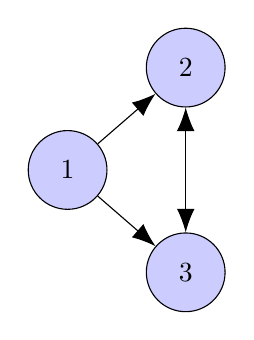
\begin{tikzpicture}[>={Latex[length=3mm]},auto, on grid, ]
      \node[main node] (1) {$1$};
      \node[main node] (2) [above right = 1.3cm and 1.5cm of 1] {$2$};
      \node[main node] (3) [below right = 1.3cm and 1.5cm of 1] {$3$};
      \draw[->] (1) edge[] node {} (2);
      \draw[->] (1) edge[] node {} (3);
      \draw[<->] (2) edge[] node {} (3);
    \end{tikzpicture}
  }
  \hfill
  \subcaptionbox{A simple undirected graph.\label{fig:graph1:b}}%
    [.3\linewidth] {
    \centering
    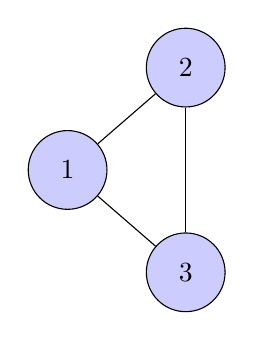
\begin{tikzpicture}[auto, on grid, ]
      \node[main node] (1) {$1$};
      \node[main node] (2) [above right = 1.3cm and 1.5cm of 1] {$2$};
      \node[main node] (3) [below right = 1.3cm and 1.5cm of 1] {$3$};
      \draw[-] (1) edge[] node {} (2);
      \draw[-] (1) edge[] node {} (3);
      \draw[-] (2) edge[] node {} (3);
    \end{tikzpicture}
  }
  \hfill
  \subcaptionbox{An undirected multigraph.\label{fig:graph1:c}}%
    [.3\linewidth] {
    \centering
    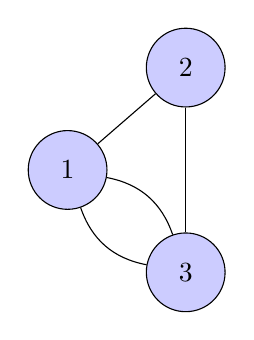
\begin{tikzpicture}[auto, on grid, ]
      \node[main node] (1) {$1$};
      \node[main node] (2) [above right = 1.3cm and 1.5cm of 1] {$2$};
      \node[main node] (3) [below right = 1.3cm and 1.5cm of 1] {$3$};
      \draw[-] (1) edge[] node {} (2);
      \draw[-] (1) edge[bend left] node {} (3);
      \draw[-] (1) edge[bend right] node {} (3);
      \draw[-] (2) edge[] node {} (3);
    \end{tikzpicture}
  }
  \caption{Examples of different graphs}
  \label{fig:graph1}
\end{figure}

Undirected graph is the opposite of directed graph in the sense that the order of the vertices in an edge does not matter:
\begin{equation}
\forall v, w \in V: (v, w) = (w, v)
\end{equation}
For example $E=\{(1, 2), (1, 2), (3, 2), (2, 3), (1, 3)\}=\{(1,2),(1,3),(2,3)\}$.
Visualization of this graph can be seen in the figure \ref{fig:graph1:b}.
For the purpose of this work, we need only undirected edges.

The definitions of graphs shown earlier do not restrict an edge to start and end in itself ($e=(v, v)$).
This kind of an edge is called a \emph{loop}.
The definition however restricts multiple same edges, \emph{parallel edges}.
In order to allow parallel edges, the edge set has to be defined as a multiset.
A graph that allows parallel edges, is called a \emph{multigraph}.
Depending on the author or context, multigraphs either allow or disallow loops.
In this work, we consider multigraphs to exist without loops.
Notice that on the figure \ref{fig:graph1:a}, there is an edge that points to both directions.
This is, in fact, not one but two edges in parallel.
It is common to visualize such cases using a two-way arrow.

A graph that has no loops or parallel edges, is called as a \emph{simple graph}.
Simple graphs can either be directed or undirected and it should be explicitly mentioned when defining graphs, unless the context implies it.
As we do not need directedness of edges, let us assume that further expressions of graphs are always undirected in this work.

For an edge $e=(v, w) \in E$ we say that $v$ is \emph{incident} to $w$ and vice versa.
If two edges share a vertex, we say that the edges are \emph{adjacent}.
The degree of a vertex is the number of edges it is connected to.
We will use the notation $\deg_G(v)$ to denote the degree of vertex $v \in V, G=(V,E)$.

A graph that is bipartite, has exactly two disjoint sets of vertices ($A$ and $B$), and every edge of the graph has one endpoint in vertex of $A$ and another in $B$:
\begin{equation}
V = A \cup B, A \cap B = \emptyset, E=\{(a, b) | a \in A, b \in B\}
\end{equation}
For bipartite graphs, the sum of degrees on A and B are equal:
\begin{equation}
\sum_{a\in A} \deg_G(a) = \sum_{b\in B} \deg_G(b)
\end{equation}
An example of a bipartite graph can be seen in the figure \ref{fig:graph2}.

\begin{figure}[h]
\centering
% https://tex.stackexchange.com/a/499577
\begin{tikzpicture}[thick,amat/.style={matrix of nodes,nodes in empty cells,
  row sep=1em,draw,dashed,rounded corners,
  nodes={draw,solid,circle}},
  fsnode/.style={fill=myblue},
  ssnode/.style={fill=myorange}]

  \matrix[amat,nodes=fsnode,label=above:$A$] (mat1) {
  1\\
  2\\
  };

  \matrix[amat,right=2cm of mat1,nodes=ssnode,label=above:$B$] (mat2) {
  3\\
  4\\
  5\\};

  \node (1) [left = of mat1-1-1] {$\deg_G(1)=2$};
  \node (2) [left = of mat1-2-1] {$\deg_G(2)=1$};
  \node (3) [right = of mat2-1-1] {$\deg_G(3)=1$};
  \node (4) [right = of mat2-2-1] {$\deg_G(4)=1$};
  \node (5) [right = of mat2-3-1] {$\deg_G(5)=1$};
  \draw (mat1-1-1) edge (mat2-1-1);
  \draw (mat1-1-1) edge (mat2-2-1);
  %\draw (mat1-2-1) edge (mat2-2-1);
  \draw (mat1-2-1) edge (mat2-3-1);
\end{tikzpicture}
\caption{A simple bipartite graph.\label{fig:graph2}}
\end{figure}

If all vertices in a graph have the same degree, then the graph is called \emph{regular}.
For example, if every vertex in a bipartite graph has the same degree, then we call it regular bipartite graph.When each part of bipartite graph is regular, we call it \emph{biregular graph}.
In fact, we use notation $(d_A,d_B)$-biregular, where $d_A$ and $d_B$ denote the degrees of the nodes inside partitions $A$ and $B$ respectively.
We can see an example of a (3,2)-biregular in the figure \ref{fig:graph3}.
The bipartite graph in the figure \ref{fig:graph2} is not biregular because the nodes in part $A$ do not share degrees i.e. $\forall v, w \in A: \deg_G(v) = \deg_G(w)$ does not hold.

\begin{figure}[h]
\centering
% https://tex.stackexchange.com/a/499577
\begin{tikzpicture}[thick,amat/.style={matrix of nodes,nodes in empty cells,
  row sep=1em,draw,dashed,rounded corners,
  nodes={draw,solid,circle}},
  fsnode/.style={fill=myblue},
  ssnode/.style={fill=myorange}]

  \matrix[amat,nodes=fsnode,label=above:$A$] (mat1) {
  1\\
  2\\
  };

  \matrix[amat,right=2cm of mat1,nodes=ssnode,label=above:$B$] (mat2) {
  3\\
  4\\
  5\\};

  \node (1) [left = of mat1-1-1] {$\deg_G(1)=3$};
  \node (2) [left = of mat1-2-1] {$\deg_G(2)=3$};
  \node (3) [right = of mat2-1-1] {$\deg_G(3)=2$};
  \node (4) [right = of mat2-2-1] {$\deg_G(4)=2$};
  \node (5) [right = of mat2-3-1] {$\deg_G(5)=2$};
  \draw (mat1-1-1) edge (mat2-1-1);
  \draw (mat1-1-1) edge (mat2-2-1);
  \draw (mat1-1-1) edge (mat2-3-1);
  \draw (mat1-2-1) edge (mat2-1-1);
  \draw (mat1-2-1) edge (mat2-2-1);
  \draw (mat1-2-1) edge (mat2-3-1);
\end{tikzpicture}
\caption{A simple (3,2)-biregular graph.\label{fig:graph3}}
\end{figure}

A graph is considered as \emph{connected} if from every node one can traverse through the edges to all other nodes i.e. every pair of nodes need to also be connected.
For instance, the graph in figure \ref{fig:graph2} has two isolated vertex subsets $\{2, 5\}$ and $\{1, 3, 4\}$, therefore the graph is not connected.
On the other hand, the graphs on figures \ref{fig:graph1:b}, \ref{fig:graph1:c} and \ref{fig:graph3} are connected.
Let's not worry about the connectivity of the directed graph on figure \ref{fig:graph1:a} as directed graphs are not relevant to this work other than in this section.


\subsection{Distributed computing} \label{sec:distributed_computing}
Computing or processing a computer program in several identical or different computers is called distributed computing
\cite{DBLP:books/el/leeuwen90/LamportL90}.
It is similiar to running a computer program that contains multiple concurrent tasks, in a computer, but in distributed computing there are higher level tasks that are distributed to different computer nodes.

Computers are called nodes, and they are connected to each other with communication channels.
These communication channels carry data from node to another node.
Together, nodes and communication channels form a network.
A common way to visualize these networks is by drawing a graph in which the nodes represent computing nodes and edges represent the communication channels.
\cite{HirvonenSuomelaDistAlg2020}

\begin{figure}[h]
  \centering
  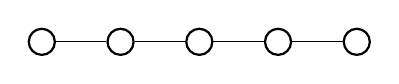
\begin{tikzpicture}[every node/.style={circle,thick,draw}]
  \node (1) {};
  \node (2) [ right of=1] {};
  \node (3) [ right of=2] {};
  \node (4) [ right of=3] {};
  \node (5) [ right of=4] {};
  \draw (1) -- (2);
  \draw (2) -- (3);
  \draw (3) -- (4);
  \draw (4) -- (5);
\end{tikzpicture}
\caption{Example of a small distributed network.}
\label{fig:dist_comp_1}
\end{figure}

According to Lamport \cite{DBLP:books/el/leeuwen90/LamportL90}, in the area of distributed computing, the term \emph{model} denotes a view or abstract representation of a distributed system.
There are multiple different computation models used in distributed computing.
The most important main category of distributed computation models is \emph{process models}.
In process models, the work or activities are represented as concurrently executed processes that execute their instructions sequentially.
The main way to distinguish different process models from each other is to categorise them by the method they use to communicate with each other (\emph{interprocess communication}).
\cite{DBLP:books/el/leeuwen90/LamportL90}


%\subsubsection{Message passing model} \label{sec:message_passing_model}
Message passing models are one form of a process model.
In the model, processes communicate by adding a message to a message queue, whether it is a shared or a process specific, and the recipient process moves the message out (dequeues) from the message queue.
\cite{DBLP:books/el/leeuwen90/LamportL90}

Different message passing models are widely used in the research field of distributed computing.
The models can varie in different details, such as in the size of the message queues \cite{DBLP:books/el/leeuwen90/LamportL90}, in the size of the messages \cite{peleg2000distributed} and on how the nodes get identified \cite{DBLP:conf/focs/Linial87}, if they are identified at all \cite{DBLP:conf/istcs/MayerNS95}.
%As the message passing models itself can be defined in multiple ways \cite{DBLP:books/el/leeuwen90/LamportL90}, we will use a definition from which the relevant models commonly inherit from.
We will dive deeper into the most relevant message passing models for this work in the following sections \ref{sec:port_number_model} and \ref{sec:local_model}.

An algorithm that is executed in a distributed fashion in a distributed network, is called as a distributed algorithm.
Each node in a network is started simultaneously and will always execute the same algorithm.
Initially the nodes are on the same state and there can be finitely or infinitely many states.
Initially the nodes are aware of only themselves and of the connections to their neighbours.
One might question that if every node starts with the same state, wouldn't they also end up in the same state?
Well yes, this happens inevitably in a case where the nodes were not given any additional symmetry breaking inputs and if every node sees the same amount of neighbours.
\cite{HirvonenSuomelaDistAlg2020}

%For example, we have a chain like network $W$ where each node $w$ has exactly two neighbours.
%The task is to execute an algorithm that finds the number of nodes in the network.


In practice, every computer node on a network has an UUID (Universally unique identifier) that can break the symmetry, and nodes are usually given some input data that they process, and nodes can always randomize data as they are never completely synchronized together, so this is not necessarily a problem.
In theory, we explicitly have to assume that there exists these kind of symmetry breaking elements.
In this works, distributed algorithms are deterministic unless otherwise mentioned.
In other research there might be randomizing involved.


\todo{Find a correct place to talk  about execution times if there is any}
In the message passing model, one could easily think that the execution time of the algorithm is the standard unit used to measure the performance but this is not true.
The message passing model implies that the dominant cost during an execution of a distributed algorithm is the message passing itself
\cite{DBLP:books/el/leeuwen90/LamportL90}.
This really... \todo{continue here}




%The following two sections (\ref{sec:port_number_model} and \ref{sec:local_model} ) talk about different forms of message passing models that are highly relative to this paper.

%In the theory of distributed computing, it is common to use terminology and concepts from graph theory as networks are basically graphs.
%With formal definitions, we can discuss more about the structure of distributed networks and reason features of those networks.
%We can further construct proofs of different theorems and so on. \todo{Fix this paragraph}

The algorithms that are executed in distributed fashion, are called distributed algorithms.
\todo{where to write about distributed algorithms?}
%A distributed algorithm is a specific type of algorithm that is executed in distributed fashion.
Specifically, each node executes the same algorithm.

%\todo{write about computation models, why they exist}


\subsubsection{Port number model} \label{sec:port_number_model}
This section is based on the course material from \cite{HirvonenSuomelaDistAlg2020} unless otherwise mentioned.

Port number model (PN model) is a rather weak model of computation that inherits from the message passing model.
In the model, nodes do not have identification.
An algorithm that executes in a port number model is called as a PN-algorithm.

We can basically take any network $N$ that has the same structure as a simple undirected graph $G$.
Each vertex of $G$ can be one-to-one mapped (bijection) to the nodes of $N$ and vice-versa.
Respectively all edges $\{v, w\}$ of $G$ can be mapped to communication channels between nodes $v$ and $w$.

Communication channels start and end from communication ports.
Each node has communication ports numbered from $1$ to $d$ where $d$ is the degree of the node.
The ports are numbered in an arbitrary order.

All nodes are considered identical, however nodes know their degree and it might differ between different nodes depending on the underlying graph $G$.
Every node starts the execution simultaneously following the same deterministic PN-algorithm $A$.
The execution of $A$ is done synchronously in parallel.
A communication round consists of following synchronous steps
\begin{enumerate}
  \item send message to each port,
  \item wait until all messages have been sent,
  \item receive a message from each port,
  \item update internal state.
\end{enumerate}
After each communication round, a node can optionally stop execution and announce its local output.
All nodes are required to eventually stop.
When all nodes have stopped, the algorithm is considered as stopped.
The running time of the algorithm $A$ is the total communication rounds that took place.








\subsubsection{Formalized port number model}
As in the previous section, this section is based on the course material from \cite{HirvonenSuomelaDistAlg2020} unless otherwise mentioned.

In the previous section \ref{sec:port_number_model} we introduced the PN model.
Now we give a formal definition of the PN model.

We call the network as a port number network or a PN-network
Port-numbering network is a 3-element tuple $N = (V, P, p)$, where $V$ and $P$ are the sets of vertices and ports respectively, and $p: P \rightarrow P$ is a function that maps a port to another port, forming a communication channel.
A port, an element of $P$, is a 2-element tuple $(v, i)$ where $v \in V$ and $i \in \{1, 2, ...\}$.
Additionally we assume that $p$ is an involution, that is, $\forall x \in P : p(p(x)) = x, $ i.e. each edge of the underlying graph is undirected.
See the figures \ref{fig:formal_pn1:a} and \ref{fig:formal_pn1:b} for examples of valid and invalid PN networks.

\begin{figure}[h]
  \subcaptionbox{A PN network of two nodes, $a$ and $b$.
    Both $a$ and $b$ have degree of 2, therefore 2 ports.
    Ports are $(a, 1), (a, 2), (b, 1)$ and $(b, 2)$.
    The connections are
      $p((a, 1)) = (b, 1)$,
      $p((a, 2)) = (b, 2)$,
      $p((b, 1)) = (a, 1)$ and
      $p((b, 2)) = (a, 2)$.
    \label{fig:formal_pn1:a}
  }%
    [.45\linewidth] {
    \centering
    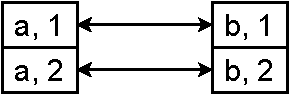
\includegraphics[scale=0.6]{diagrams/formalizing_pn_network_diagram1.pdf}
  }
  \hfill
  \subcaptionbox{
    An invalid PN network as port mapping function $p$ is not an involution:
    $p(p((a, 1))) = p(p((a, 2))) \neq (a, 1)$.
    \label{fig:formal_pn1:b}
  }%
    [.45\linewidth] {
    \centering
    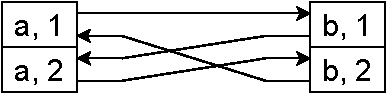
\includegraphics[scale=0.6]{diagrams/formalizing_pn_network_diagram2.pdf}
  }
  \caption{Examples of a valid and an invalid PN network.}
  \label{fig:formal_pn1}
\end{figure}


The degree $\deg_N(v)$ of a node $v \in V$ is equal to the number of ports of $v$.
We assume that the port numbers are consecutive positive integers starting from 1, i.e. the ports of a node $v$ are $\{(v, i) | i \in \{1, 2, ..., \deg_N(v)\}\}$.
Note that the highest port number of $v$ is also the degree of $v$.

When we say \emph{port number $i$ in node $v$}, we refer to the port $(v, i)$.
When we say \emph{port $(v, i)$ is connected to port $(w, j)$}, we refer to $p((v, i)) = (w, j)$.

A loop is a connection where port $(v, i)$ is connected to port $(v, j)$.
For example there are two loops, p((a, 1)) = p((a, 2) and p((c,2)) = (c,2), in the figure \ref{fig:formal_pn2:c}.

There are multiple connections between two distinct nodes $v$ and $w$, if $p((v, i_1)) = (w, j_1)$, $p((v, i_2)) = (w, j_2)$, $i_1 \neq j_1$ and $i_2 \neq j_2$.
For example the connections $p((b, 2)) = (d, 1)$ and $p((b, 3)) = (d, 2)$ in the figure \ref{fig:formal_pn2:c}.

If a PN network has neither loops or multiple connections, it is called a \emph{simple} network.
For example the network is simple in the figure \ref{fig:formal_pn2:a}.

Each simple PN network $N=(V,P,p)$ also has a thing called an underlying graph $G=(V,E)$.
An edge $(v, w)$ is part of the underlying network if and only if $v$ and $w$ are connected, that is, $E = \{ \{v, w\} \, | \,  p((v, i)) = (w, j) \}$ where ${v, w} \in E$.

\begin{figure}[h]
  \subcaptionbox{
    A simple PN network.
    The underlying graph is also simple.
    \label{fig:formal_pn2:a}
  }%
    [.3\linewidth] {
    \centering
    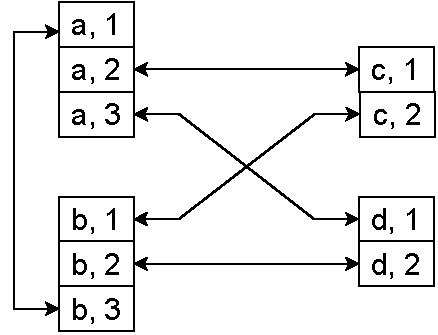
\includegraphics[scale=0.6]{diagrams/formalizing_pn_network_diagram4.pdf}
  }
  \hfill
  \subcaptionbox{
    An alternative representation of the PN network from figure \ref{fig:formal_pn2:b}
    \label{fig:formal_pn2:b}
  }%
    [.3\linewidth] {
    \centering
    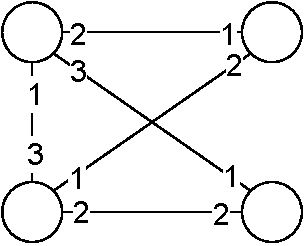
\includegraphics[width=0.3\textwidth]{diagrams/formalizing_pn_network_diagram5.pdf}
  }
  \hfill
  \subcaptionbox{
    A PN network with loops and parallel connections.
    This kind of network cannot be shown in the alternative representation unlike the network on figure \ref{fig:formal_pn2:a}.
    \label{fig:formal_pn2:c}
  }%
    [.3\linewidth] {
    \centering
    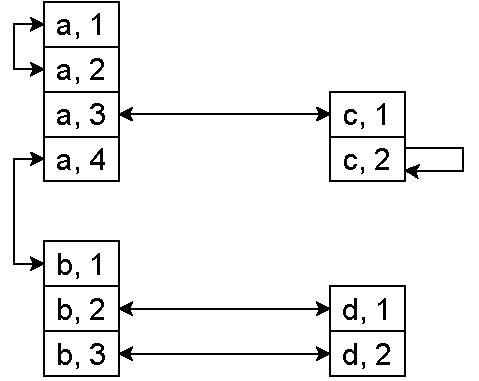
\includegraphics[scale=0.6]{diagrams/formalizing_pn_network_diagram3.pdf}
  }
  \caption{Examples of simple and non simple PN networks.}
  \label{fig:formal_pn2}
\end{figure}


%\todo{continue from here on  TUESDAY 4.1.2022}



\todo{Add formal definition of the PN algorithm}
Port numbering algorithm is ...



\subsubsection{LOCAL model} \label{sec:local_model}

\subsection{LCL problems} \label{sec:lcl_problems}

\subsection{Boolean satisfiability problem}

\subsection{Previous research} \label{sec:previous_research}

\todo{Especially LCL classification research}

\clearpage



\clearpage
%!tex root = ../main.tex

\section{Research questions} \label{sec:research_question}

There are LCL problems that cannot be solved in the PN model.
More specifically, there exist LCL problems such that no PN algorithm can solve it in \emph{every} PN network.
Therefore, if an LCL problem is unsolvable in the PN model, then there exists no valid labeling to the problem for some PN network.
We are interested in detecting the unsolvability of an LCL problem automatically.

\begin{researchquestion} \label{research_question:1}
Given an LCL problem, how can we automatically detect the unsolvability of the problem in the PN model?
\end{researchquestion}

We answer to Research question \ref{research_question:1} in Section \ref{sec:algorithm}, where we present our algorithm that can automatically detect the unsolvability of an LCL problem in the PN model.

In Section \ref{sec:algorithm}, we present Theorem \ref{thm:lcl_unsolvability}, which says that an unsolvability of an LCL problem in the PN model implies that the problem is also not solvable in constant time in the LOCAL model.
We want to know if we can prove it.

\begin{researchquestion} \label{research_question:2}
Can we prove that an unsolvability of an LCL problem in the PN model implies that the problem is also not solvable in constant time in the LOCAL model?
\end{researchquestion}

As our answer to Research question \ref{research_question:2}, we prove Theorem \ref{thm:lcl_unsolvability} in Section \ref{sec:algorithm:prooving_the_theorem}.
The proof relies on multiple lemmas that we introduce in Sections \ref{sec:algorithm:from_multiple_to_simple} and \ref{sec:algorithm:from_pn_to_local}.

We have implemented the algorithm from Section \ref{sec:algorithm} that we give as an answer to Research question \ref{research_question:1}, and we introduce details of the implementation in Section \ref{sec:implementation}.
With Theorem \ref{thm:lcl_unsolvability}, the results from the tool can be derived to non-constant lower bounds in the LOCAL model.
There also exists a database of upper and lower bounds of LCL problems \cite{Tereshchenko2021}, and these bounds have been computed using various tools called \emph{classifiers}.
Our implementation is one kind of classifier, and we want to know if it can find any new lower bounds i.e. lower bounds that are higher than what is currently known about these problems.

\begin{researchquestion} \label{research_question:3}
Using our implementation, for which LCL problems can we determine new lower bounds in the LOCAL model?
\end{researchquestion}

The algorithm can be run with a single problem, but we also want to target classes of problems, where the quantity of problems can be large.
Thus, we want our implementation to be reasonable fast in order it to have use in practice.

\begin{researchquestion} \label{research_question:4}
Can we make the implementation fast enough, so that we can classify interesting problem classes in practice?
\end{researchquestion}

As an answer to Research questions \ref{research_question:3} and \ref{research_question:4}, we present the results from our implementation in Section \ref{sec:results}.
The results will include new problem classifications, execution time statistics and ... \todo{Complete these after results are done.}.
%TODO


\clearpage
%!tex root = ../main.tex

\section{Prior work} \label{sec:prior_work}
%In this section, we discuss the related studies that have been released prior to this work.
%\todo{\(\leftarrow\) is this sentence needed?}
In computer science, we are often interested in finding the best possible algorithm for some computational problem.
First, in Section~\ref{sec:prior_work:automation_of_proving}, we generally discuss the \emph{automation of finding} information about the best possible algorithm, and we briefly discuss what has been previously done related to the subject, in the field of computer science.
In Section~\ref{sec:prior_work:automation_of_proving_in_local_model} we narrow our focus on the subject to the field of distributed computing.
In addition, we will discuss relevant automated tools that have been developed prior this work and the complexity classes that are relevant in the LOCAL model.

\subsection{Automation of proving} \label{sec:prior_work:automation_of_proving} %Algorithm synthetization
%\todo{Maybe start talking more generally, without mentioning anything about LOCAL or LCL, and explain that in computer science, we are looking for }
Given that we have an interesting computational problem, our ultimate end goal is to find the best possible (i.e. optimal) algorithm for the computational problem.
We would like to learn something new about the computability of the problem in terms of computational complexity, in order to narrow the search for the best algorithm.
There are usually two desirable results we would want to discover.
\begin{itemize}
    \item
    The first desirable result is an efficient algorithm that solves the computational problem.
    The existence of such algorithm would show that the problem is solvable with \emph{at least} at the efficiency of the algorithm.
    \item
    The second desirable result would be the information that such efficient algorithm does not exist at all.
    If there are provably no algorithms with such efficiency, then possible algorithms have to be \emph{less} efficient.
\end{itemize}
We say that the former results, showing existence, an upper bound, or possibility, are \emph{positive} results.
Similarly, the latter results, showing nonexistence, a lower bound, or impossibility, are \emph{negative} results.
In our work, the objective is to find negative results, but we would also like to briefly discuss finding positive results as it is the other side of discovering new information about the computability of computational problems.

Traditionally, positive and negative results for computational problems have been found using the pen-and-paper method.
For example, Linial\ \cite{DBLP:conf/focs/Linial87} showed in 1987 that there is a deterministic \(\mathcal{O}(\log^* n)\) algorithm for \(\mathcal{O}(\Delta^2)\)-coloring.
In a more recent paper from 2010, Barenboim and Elkin\ \cite{DBLP:conf/podc/BarenboimE10} showed that there is a deterministic \emph{polylogarithmic} time algorithm for \(\Delta^{1 + o(1)}\)-coloring, which is substantially better in terms of the quantity of colors, in comparison to the former paper \cite{DBLP:conf/focs/Linial87} from Linial.

A more recent approach to finding positive or negative results is the \emph{automation} of the whole process.
One could automate the finding of positive or negative results by utilizing massive computational power of modern computers.
The case of negative results is exactly one of our work's objectives, and we will discuss the automation of finding these results in the distributed computing in Section \ref{sec:prior_work:automation_of_proving_in_local_model}.
But first, what about the automation of finding positive results?

The automation of finding positive results involves creating a tool that takes a specification of desired behavior as an input, and outputs an algorithm that matches the specification, and this method is called \emph{algorithm synthesis} \cite{DBLP:phd/basesearch/Rybicki16}.
For example, in the work of Dramnesc and Jebelean from 2015, the authors manage to automatically synthesize various sorting algorithms including selection sort, insertion sort, quick sort, merge sort and a novel sorting algorithm they call \emph{unbalanced merge sort} \cite{DBLP:journals/jsc/DramnescJ15}.
As another example, in the work of Gulwani et~al. from 2011, the authors present a tool that can efficiently synthesize highly nontrivial 10--20 line loop-free bit vector programs \cite{DBLP:conf/pldi/GulwaniJTV11}.

Propositional satisfiability solvers (SAT solvers) have been used in various synthesis problems to find positive results.
SAT solvers are also used in our implementation to find negative results, and we will talk more about them in Section \ref{} (\todo{Add reference to section where we explain SAT}), but nevertheless we will next show an examples of a previous research.
SAT solvers have been used especially in synthesis of circuits, where one goal is to find optimal Boolean circuits in terms of size.
As the example, in the paper from Järvisalo et al.\ \cite{DBLP:conf/sat/JarvisaloKKK12}, the authors present a method to encode an ensemble computation problem as a propositional formula.
The encoding is then fed to a SAT solver to gain either a working circuit design for the ensemble computation problem or a proof of nonexistence.

%\todo{algorithm synthesis is by no means easy, it is often undecidable or bla bla bla, check the väikkäri}
%"given a specification of the desired behavior, let the computer find an algorithm that matches the specification"\cite{DBLP:phd/basesearch/Rybicki16}

\subsection{Automation of proving in the LOCAL model} \label{sec:prior_work:automation_of_proving_in_local_model}


A tool that automates the finding of positive or negative results in distributed computing is called \emph{classifier}.
A classifier can automatically determine a lower bound or an upper bound for an LCL problem.
Currently, we are aware of only small number of different classifiers, and we will list them below in Table \ref{tbl:classifiers}.
These classifiers work in the LOCAL model, meaning that the results outputted by the classifiers are time complexities in the LOCAL model.

Generally, there are infinitely many complexity classes because there are infinitely many functions.
However, in the LOCAL model, infinitely many of them turns out to be redundant.
\emph{Gap theorems} show that there are ranges of complexities where there exists no optimal algorithms for LCL problems.
For example, Balliu et~al.~\cite{DBLP:conf/podc/BalliuHOS19} showed that the deterministic complexity of an optimal algorithm is either at most \(\mathcal{O}(1)\) or requires at least \(\Omega(\log^* n)\) rounds.
As another example, Chang et~al.~\cite{DBLP:conf/focs/ChangKP16} showed that there is a gap between \(\mathcal{O}(\log^* n)\) and \(\Omega(\log n)\).
Currently, the main complexities we care about, in the deterministic LOCAL model, are the following:
\[\mathcal{O}(1), \Theta(\log^* n), \Theta(\log n), n^{\Theta(1)}.\]
This is the reason why the output complexity for an LCL problem, from a classifier, is typically one of these 4 complexities.

\begin{table}[H]
\centering
\begin{threeparttable}[t]
\begin{adjustbox}{width={\textwidth},keepaspectratio}%
\begin{tabular}{l l l l l l l}
    \toprule
    &&&&& \multicolumn{2}{c}{Trees} \\
    \cmidrule{6-7}
    Classifier & Complete & Labels & Paths & Cycles &Rooted & Unrooted \\\midrule
    %
    poly-classifier \cite{PolyClassifier2022, DBLP:journals/corr/abs-2202-08544}
    & Yes\tnote{1} & Any & No & No & Yes\tnote{2} & Yes\tnote{2} \\
    %
    Rooted tree classifier \cite{RootedTreeClassifier2021, DBLP:conf/podc/Balliu0OSST21}
    & Yes & Any & No & No & Yes\tnote{2} & No \\
    %
    Automata-theoretic lens classifier \cite{CyclePathClassifier2020, DBLP:conf/sirocco/ChangSS21}
    & Yes & Any & Yes & Yes & No\tnote{3} & No \\
    %
    Round Eliminator \cite{DBLP:conf/podc/Olivetti20, OlivettiRoundEliminatorGithub, DBLP:conf/podc/Brandt19}
    & No & Any\tnote{4} & Yes & No &  No & Yes \\
    %
    Tree-classifications (dataset) \cite{TreeClassifications2020}
    & No & 2, 3 & No & No & No  & Yes \\
    %
    TLP Classifier \cite{RocherTlpClassifier2020, Rocher2020}
    & No & 3 & Yes & No & No  & Yes \\ \bottomrule
    %
\end{tabular}%
\end{adjustbox}
\begin{tablenotes}[normal,flushleft]
    \footnotesize
    \item[1] Complete only in rooted trees.
    \item[2] Only in binary trees. In theory, it applies to all regular trees.
    \item[3] The paper~\cite{DBLP:conf/sirocco/ChangSS21} shows that it applies to some LCL problems in rooted trees.
    \item[4] Up to \(\frac{64}{\Delta}\).
\end{tablenotes}
\end{threeparttable}
\caption{A list of all classifiers we are aware of prior this work.} \label{tbl:classifiers}
\end{table}

In Table \ref{tbl:classifiers}, we list for each classifier the graph families they target to, the amount of labels they support and the completeness.
We define classifier as \emph{complete} if it can output a tight complexity class, from the previous list of 4 main complexities, for any input problem in the problem class it targets to.
There are multiple reasons for a classifier to be \emph{incomplete}, including:
\begin{itemize}
    \item it only outputs either upper or lower bound,
    \item it outputs ``no result'' i.e. it does not know the complexity class,
    \item it does not terminate.
\end{itemize}
Our classifier works only with unrooted trees and is incomplete in the sense that it gives only lower bounds, and only for some LCL problems.
In the table, we list the number of labels each classifier supports, and by `Any' we mean that a classifier supports reasonably high quantity of labels.


\clearpage
%!tex root = ../main.tex

\section{Algorithm} \label{sec:algorithm}

In this section, we will introduce the basic idea of an essential algorithm that is used in the actual implementation discussed in section \ref{sec:implementation}.
The algorithm's purpose is to find a proof that a given LCL problem $\Pi$ is impossible to solve in PN model.
Here we specifically allow PN networks to have multiple connections.
Later in the Section \ref{sec:algorithm:theorems:a} we show that the unsolvability of a problem $\Pi$ in PN networks (with multiple connections) implies that it is also impossible to solve $\Pi$ in \emph{simple} PN networks (without multiple connections).
Finally in the Section \ref{sec:algorithm:theorems:b} we show that the unsolvability of $\Pi$ in \emph{simple} PN networks implies that $\Pi$ is not solvable in constant time ($\mathcal{O}(1)$) in the LOCAL model.

First we start with defining the meaning of solvability of an LCL problem.
%TODO These definitions and theorems might have a better place under section 2 background.
\begin{definition} \label{def:lcl_solvability}
    An LCL problem $\Pi$ is solvable in PN model, if and only if there exists a PN algorithm $A$ that finds a solution for $\Pi$ in all PN networks.
\end{definition}

We can define an alternative version of the Definition \ref{def:lcl_solvability} using contraposition.
\begin{definition} \label{def:lcl_solvability:contrapositive}
An LCL problem $\Pi$ is not solvable in PN model, if and only if there does not exist a PN algorithm $A$ that finds a solution for $\Pi$ in all PN networks.
\end{definition}

The Definitions \ref{def:lcl_solvability} and \ref{def:lcl_solvability:contrapositive} are equivalent. The latter one might be more difficult to understand, but the way it is phrased, easily leads us to the following Theorem:

\begin{theorem} \label{thm:lcl_nonsolvability}
    An LCL problem $\Pi$ is not solvable in PN model, if there exists a PN network $N$ such that no PN algorithm $A$ can solve the $\Pi$ in $N$.
\end{theorem}
\begin{proof}
    Let $\Pi$ be an LCL problem.
    Let $N$ be a PN network such that no PN algorithm $A$ can solve $\Pi$ in $N$.
    Therefore no PN algorithm $A$ can find a solution to $\Pi$ in all PN networks.
    According to the definition \ref{def:lcl_solvability:contrapositive}, this is equivalent with $\Pi$ being unsolvable.
\end{proof}

As the Theorem \ref{thm:lcl_nonsolvability} shows us, to show that a problem $\Pi$ is unsolvable, it is enough to find a counterexample, a PN network $N$ in which the problem $\Pi$ cannot be solved.
To show that, it is enough to find an underlying graph $G$ of $N$ in which the problem $\Pi$ cannot be solved.
\begin{theorem} \label{thm:problem_nonsolvability_in_graphs}
    If a problem $\Pi$ is not solvable in graph $G$, then $\Pi$ is also not solvable in any PN network $N$ that has $G$ as its underlying graph.
\end{theorem}
\begin{proof}
\todo{Complete proof} %TODO complete proof
\end{proof}

Using this fact, we can come up with an algorithm that automatically tries to find an counterexample graph.

\begin{algorithm}[H]
    \caption{Counterexample graph finder algorithm}
    \label{alg:counterexample_finder}
    \begin{algorithmic}[1] % The number tells where the line numbering should start
        \Require $1 \leq n_{low} \leq n_{high}$
        %\Require $\Pi$ is an LCL problem
        \Function{Find}{$n_{low},n_{high}, \Pi$} \Comment{Graph bounds $n_{low}$ and $n_{high}$, LCL problem $\Pi$} \label{alg:counterexample_finder:n_loop}
            \State $d_a \gets \textsc{ActiveDegree}(\Pi)$ \label{alg:counterexample_finder:d_a}
            \State $d_p \gets \textsc{PassiveDegree}(\Pi)$ \label{alg:counterexample_finder:d_p}
            \For{$n\gets n_{low}, n_{high}$} \Comment{Iterate graph sizes from lowest to highest} \label{alg:counterexample_finder:n}
                \State $G_n \gets \textsc{GenerateGraphs}(n, d_a, d_p)$ \label{alg:counterexample_finder:Gn}
                \ForEach{$g \in G_n$} \label{alg:counterexample_finder:g}
                    \If {$\textsc{IsUnsolvable}(\Pi, g)$} \label{alg:counterexample_finder:is_unsolvable}
                        \State \Return $g$ \label{alg:counterexample_finder:return_g}
                    \EndIf
                \EndFor
            \EndFor
            \State \Return \Comment{No counterexample found. Return nothing.} \label{alg:counterexample_finder:return_nothing}
        \EndFunction
    \end{algorithmic}
\end{algorithm}

The Algorithm \ref{alg:counterexample_finder} is designed to find the smallest counterexample graph for an LCL problem $\Pi$.
It starts from graphs with $n_{low}$ vertices and goes up to graphs with $n_{high}$ vertices.
We define $d_a$ and $d_p$ to be the active and passive degree of the problem $\Pi$ respectively (rows \ref{alg:counterexample_finder:d_a} and \ref{alg:counterexample_finder:d_p}).
The variable for the current vertex count is called $n$ (row \ref{alg:counterexample_finder:n}).
For each graph with $n$ vertices, we generate all possible $(d_a, d_p)$-biregular multigraphs with $\textsc{GenerateGraphs}(n, d_a, d_p)$, and save the graphs into variable $G_n$ (row \ref{alg:counterexample_finder:Gn}).
The reason for generating only these types of graphs comes from our definition of LCL problem from section \ref{sec:lcl_problems}, they are defined specifically for $(b,a)$-biregular (multi)graphs.
%TODO make sure that it defines the LCL problems we are using here (LCL for (b,a)-biregular graphs)
Now, for each graph $g \in G_n$ (row \ref{alg:counterexample_finder:g}) we check if the given problem $\Pi$ is unsolvable using the function $\textsc{IsUnsolvable}(\Pi, g)$ (row \ref{alg:counterexample_finder:is_unsolvable}).
If it is unsolvable, we return the graph as an counterexample (row \ref{alg:counterexample_finder:return_g}).
In the case there are no counterexamples in graphs with $n_{low}$ to $n_{high}$ vertices, the algorithm returns nothing (row \ref{alg:counterexample_finder:return_nothing}).

Up to this moment, we have not discussed about how the function $$\textsc{GenerateGraphs}(n, d_a, d_p)$$ from row \ref{alg:counterexample_finder:Gn} generates the graphs, nor have we discussed about how the function $$\textsc{IsUnsolvable}(\Pi, g)$$ from row \ref{alg:counterexample_finder:is_unsolvable} determines the unsolvability used in the Algorithm \ref{alg:counterexample_finder}.
These functions are implementation specific and in this section we assume that they exist as black boxes.
Later on the section \ref{sec:implementation} we introduce our implementations of these functions.
%First we would like to discuss about the $\textsc{GenerateGraphs}(n)$.
%As we know from the section \ref{}, %TODO refer to LCL section and make sure that it defines the LCL problems we are using here (LCL for (b,a)-biregular graphs).
%the LCL problems used in this thesis are defined for $(b,a)$-biregular graphs.
%Therefore we should not generate \emph{all} graphs but only the graphs of type $(b,a)$-biregular, where the degrees $b$ and $a$ are taken from the LCL problem $\Pi$.



%TODO talk about graphs, why they are actually (b, a)-biregular multigraphs. Maybe this is explained by the fact that our LCL problems are defined for (b, a)-biregular.
%TODO talk about networks and graphs. In the above text they are refered as if they were the same thing.
%TODO Do we need to talk about trees and how these biregular multigraphs relate to them? 'Informally, the idea is to prove negative results for the case in which "we are in the middle of a very large tree, far away from the leaves".'

In the following sections, we will prove that if an LCL problem $\Pi$ is not solvable in PN network $N$ with multiple connections, then it is not solvable in constant time in the LOCAL model.
We have divided the proofs into multiple theorems and grouped them under two different sections, Section \ref{sec:algorithm:theorems:a} and Section \ref{sec:algorithm:theorems:b}.
The dependencies of theorems are shown in the Figure \ref{fig:algorithm:theorem_dependency}.
\footnote{Where should I put these theorems? Do they fit under Section \ref{sec:algorithm}?}

\begin{figure}[H]
    \centering
    % https://tex.stackexchange.com/a/499577
    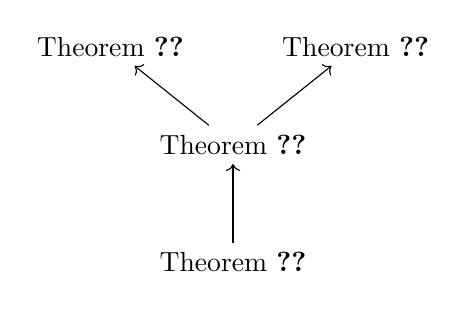
\begin{tikzpicture}[]
        \node (1) [] {Theorem \ref{thm:lcl_nonsolvability:2}};
        \node (2) [right = of 1] {Theorem \ref{thm:lcl_nonsolvability:3}};
        \node (3) [below = of $(1)!0.5!(2)$] {Theorem \ref{thm:lcl_nonsolvability:4}};
        \node (4) [below = of 3] {Theorem \ref{thm:lcl_nonsolvability:5}};
        %\node (4) [right = of mat2-2-1] {$\deg_G(4)=2$};
        %\node (5) [right = of mat2-3-1] {$\deg_G(5)=2$};
        \draw[<-] (1) edge (3);
        \draw[<-] (2) edge (3);
        \draw[<-] (3) edge (4);
    \end{tikzpicture}
    \caption{A dependency graph of the following theorems.\label{fig:algorithm:theorem_dependency}}
\end{figure}

\subsection{\todo{Theorems A}} \label{sec:algorithm:theorems:a}
In this section we show that if an LCL problem is not solvable in PN networks with multiple connections, then the problem is also not solvable in simple PN networks.
We try to split this into couple of theorems and at the end utilize the shown theorems to show this to be true.

% Pi is nonsolvable in multiple connection PN network N -> Pi is nonsolvable in lift of N
\begin{theorem} \label{thm:lcl_nonsolvability:2}
If an LCL problem $\Pi$ is not solvable in PN network $N$, then it is also not solvable in any PN network $N'$ that is a lift of $N$.
\end{theorem}
\begin{proof}
    Let problem $\Pi$ have no solution in some PN network $N$.
    Then any algorithm $A$ produces a result that is nonvalid solution to $\Pi$ i.e. a local constraint is violated at least at some node $v$.
    Let $\phi: V' \rightarrow V$ be a covering map from $N'=(V', P', p')$ to $N=(V, P, p)$.
    Theorem 7.1. \footnote{\todo{should I show the theorem or is this enough?}} from the text book \cite{HirvonenSuomelaDistAlg2020} shows that the nodes of $N'$ will have exactly the same state as their counterparts at $N$ for each time unit $t=0,1,...$.
    Hence if we run algorithm $A$ on both networks $N$ and $N'$, the local constraint violation at some node $v \in N$ also appears in all nodes $v' \in V'$ such that $\phi(v') = v$ i.e. the local constraint violations also appear in the covering network $N'$.
\end{proof}

% Network with multiple connections ----k-lift--->  simple network
\begin{theorem} \label{thm:lcl_nonsolvability:3}
    If there is a PN network $N_2$ with multiple connections with $k$ being the highest count of multiple connections between any two nodes, then there exists a $k$-lift $N_1$ of $N_2$ such that $N_1$ is a simple PN network.
\end{theorem}
\begin{proof}
    Let $N_2=(V_2, P_2, p_2)$ be a PN network with multiple connections.
    Let $\operatorname{mul}(u, v)$ be the number of connections between any nodes $u, v \in V_2$.
    Let $k=\max (\{ m(u, v) \mid u, v \in V_2\} )$ i.e. the highest count of multiple connections.
    \footnote{\todo{Is the "maximum number of multiple connections" ambiguous? Does it appear as the highest count of parallel connections or as the total number of multiple connections in the network?}}
    Let $\operatorname{M}(x+hk) = x$ for all $x = 1, ..., k$ and $h\in \mathbb{N}$, for example $\operatorname{M}(1 + hk) = 1$ and $\operatorname{M}(k + hk) = k$.

    Let there be another network $N_1=(V_1, P_1, p_1)$ such that:
    \begin{itemize}
        \item For each $v \in V_2$, there are $k$ clones in $V_1$, namely the nodes $v_1, v_2, ..., v_k \in V_1$.
        Thus the sizes $|V_1|$ and $k|V_2|$ are equal.
        %$V_1 = \{v_x: \forall v \in V_2, \forall x \in \{1, 2, ..., k\}\}$
        \item For each port $(v, i) \in P_2$, we have each port $(v_x, i) \in P_1$ where $x=1, 2, ..., k$.
        %% TODO remove these comments when this has been reviewed.
        %\item For each non-multiple connection $p_2((v, i)) = (u, j)$, we have connections $p_1((v_x, i)) = (u_x, j)$, where $x=1, 2, ..., k$.
        %\item For each multiple connections $p_2((v, i_a)) = (u, j_a)$ where $a = 1, 2, ..., \operatorname{mul}(u, v)$, we have $p_1((v_{x}, i_a)) = (u_{\operatorname{M}(x+a-1)}, j_a)$.
        %Note that the non-multiple connections are just a special case where $a$ is always $1$.

        \item For each connection $p_2((v, i_a)) = (u, j_a)$ where $a = 1, 2, ..., \operatorname{mul}(u, v)$, we have $p_1((v_{x}, i_a)) = (u_{\operatorname{M}(x+a-1)}, j_a)$.
        Note that if $\operatorname{mul}(u, v) = 1$, then $p_1((v_{x}, i_1)) = (u_{\operatorname{M}(x)}, j_1) = (u_{x}, j_1)$.
    \end{itemize}

    Now we show that there is a covering map $\phi: V_1 \rightarrow V_2$.
    Let $\phi(v_x) = v \in V_2$ for each $v_x \in V_1$ where $x=1, 2, ..., k$.
    We will show that $\phi$ is a covering map using the Definition \ref{def:covering_map}:
    \begin{itemize}
        \item By the definition of $\phi$, it is surjective.
        \item For each connection in $N_2$, we have $k$ similiar connections in $N_1$, therefore degrees of each node are preserved.
        %% TODO remove these comments when this has been reviewed.
        %\item For each non-multiple connection $p_1((v_x, i)) = (u_x, j)$, where $x=1, 2, ..., k$, we have $p_2((v, i)) = (u, j)$.
        %From our definition of $\phi$ we can see that the mapping preserves port numbers and connections in non-multiple connections.
        %\item For each multiple connection $p_1((v_{x}, i_a)) = (u_{\operatorname{M}(x+a-1)}, j_a)$ we have
        %\begin{align*}
        %    p_2((\phi(v_{x}), i_a)) &= (\phi(u_{\operatorname{M}(x+a-1)}), j_a)\\
        %    \Leftrightarrow p_2((v, i_a)) &= (u, j_a)
        %\end{align*}
        %Both $(v, i_a)$ and $(u, j_a)$ are in $P_2$ and $p_2((v, i_a)) = (u, j_a)$, therefore for each multiple connection, the port numbers and connections are preserved.
        \item For each connection $p_1((v_{x}, i_a)) = (u_{\operatorname{M}(x+a-1)}, j_a)$ we have
        \begin{align*}
           p_2((\phi(v_{x}), i_a)) &= (\phi(u_{\operatorname{M}(x+a-1)}), j_a)\\
           \Leftrightarrow p_2((v, i_a)) &= (u, j_a)
        \end{align*}
        Both $(v, i_a)$ and $(u, j_a)$ are in $P_2$ and $p_2((v, i_a)) = (u, j_a)$, therefore for each connection, the port numbers and connections are preserved.
    \end{itemize}
    Each condition holds, hence the function $\phi$ is a covering map from $V_1$ to $V_2$
    therefore $N_1$ is a $k$-lift of $N_2$.

    We need to show that $N_1$ is a simple PN network i.e. it does not have multiple edges.
    %As we know, the non-multiple connections in $N_2$ are preserved in $N_1$ therefore we need to only look at the multiple connections of $N_2$ in more detail.
    We know that there are connections $p_1((v_{x}, i_a)) = (u_{\operatorname{M}(x+a-1)}, j_a)$ where $a=1, 2, ..., \operatorname{mul}(\phi(v_{x}),\phi(u_{\operatorname{M}(x+a-1)}))$.
    We see that nodes $u_{\operatorname{M}(x+a-1)}$ are distinct for all $a$ because $1 \leq a \leq \operatorname{mul}(\phi(v_{x}),\phi(u_{\operatorname{M}(x+a-1)})) \leq k$ and
    there are exactly k many "u" nodes in $V_1$, namely nodes $u_1, u_2, ..., u_k \in V_1$.
    Thus for each node $v_x$, all connections from $v_x$ are mapped to distinct nodes, therefore $N_1$ is simple.

    The network $N_2$ is connected by the assumption (Section \ref{sec:underlying_graph}) but it might not be clear that $N_1$ is connected, thus we show next that this is the case.

    Let us look at all connections in $p_1$ and fix $a=1$.
    Then $p_1((v_{x}, i_a)) = (u_{\operatorname{M}(x+a-1)}, j_a)$
    $=p_1((v_{x}, i_1)) = (u_{x}, j_1)$.
    This shows that we can traverse from any node $w_x\in P$ to any other node $w'_x\in P$ only using nodes with subscript $x$.

    There are at least some nodes $u, v \in P_2$ such that $\operatorname{mul}(u,v) = k$, therefore we can traverse from any $u_x \in P_1$ to any $v_y \in P_1$ for any $x, y \in \{1, 2, ..., k\}$.
    Thus $N_1$ is connected.
\end{proof}

%\begin{figure}[H]
% \centering
% \includegraphics[]{example-image-duck}
% \caption{\todo{Illustration of k-lift using Theorem \ref{thm:lcl_nonsolvability:3}}}
% \label{fig:duck2}
%\end{figure}

\begin{figure}[H]
    \subcaptionbox{
      A PN network $N_2$ with multiple connections.
      \label{fig:algorithm:k-lift_proof_simple1:a}
    }%
      [.5\linewidth] {
      \centering
      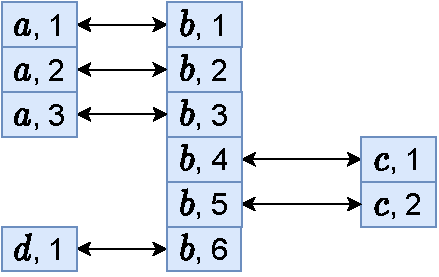
\includegraphics[scale=0.55]{diagrams/algorithm_k-lift_proof_simple_1.pdf}
    }
    \hfill
    \subcaptionbox{
      A simple PN network $N_1$.
      \label{fig:algorithm:k-lift_proof_simple1:b}
    }%
      [.5\linewidth] {
      \centering
      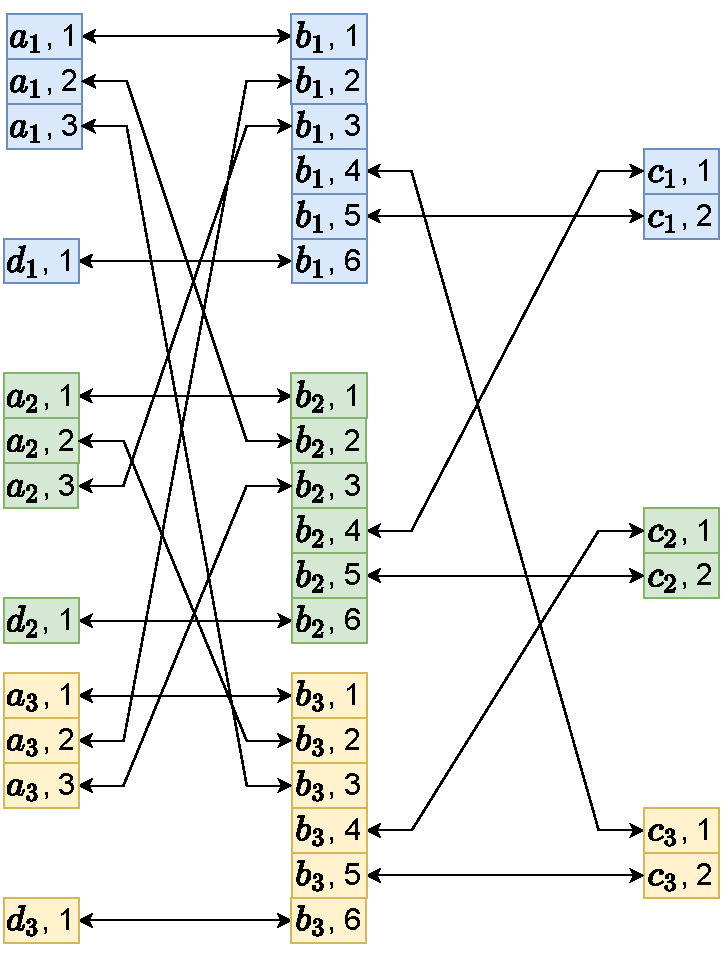
\includegraphics[scale=0.55]{diagrams/algorithm_k-lift_proof_simple_2.pdf}
    }
    \caption{The network $N_1$ is a 3-lift of the network $N_2$.
    }
    \label{fig:algorithm:k-lift_proof_simple1}
  \end{figure}


%% This is more like an instruction on how to build the network, not a proof or is it?

    % Let $N=(V, P, p)$ be a PN network with multiple connections.
    % Let $m(u, v)$ be the number of connections between any nodes $u, v \in V$.
    % Let $k=\max {m(u, v) | u, v \in V}$ i.e. the maximum number of multiple connections.
    % \footnote{\todo{Is the "maximum number of multiple connections" ambiguous? Does it appear as the highest count of parallel connections or as the total number of multiple connections in the network?}}

    %Let's construct a new network $N'=(V', P', p')$ that consists of $k$ copies of $N$.
    %Initially the network $N'$ is not connected and therefore it is not a valid PN network but lets ignore this for now as the network gets valid soon as we alter it.
    %For each connection (v', j')
%
    %Let $\phi: V' \rightarrow V$ be a surjection such that for each node $v_i \in V'$ where $i=1, 2, ..., k$, $\phi(v_i) = v \in V$.
    %Next, we will swap the ends of connections such that the network becomes connected and
    %\todo{Complete this proof}
% Pi is nonsolvable in multiple connection PN network N -> Pi is nonsolvable in simple PN network N' (lift of N)
\begin{theorem} \label{thm:lcl_nonsolvability:4}
    If an LCL problem $\Pi$ is not solvable in PN network $N_2$ with multiple connections, then it is also not solvable in simple PN network $N_1$ that is a lift of $N_2$.
\end{theorem}
\begin{proof}
    Let us assume that an LCL problem $\Pi$ is not solvable in PN network $N_2$ with multiple connections.
    Theorem \ref{thm:lcl_nonsolvability:3} shows that there exists a k-lift $N_1$ of $N_2$ such that $N_1$ is a simple PN network.
    Theorem \ref{thm:lcl_nonsolvability:2} shows that the problem $\Pi$ is also not solvable in network $N_1$.
    Therefore the problem $\Pi$ is not solvable in simple PN network $N_1$ that is a lift of $N_2$.
\end{proof}

\subsection{\todo{Theorems B}} \label{sec:algorithm:theorems:b}


\begin{theorem} \label{thm:lcl_nonsolvability:5}
    If a problem is not solvable in simple PN networks, then it is not solvable in constant ($\mathcal{O}(1)$) time in the LOCAL model.
    %TODO Make sure that the LOCAL model is explained under section 2. background.
    %TODO Make sure that the solving complexities (($\mathcal{O}(1)$) time) are explained under section 2. background.
\end{theorem}
\begin{proof}
    \todo{Complete this proof} %TODO Complete this proof
\end{proof}

\clearpage
%!tex root = ../main.tex

%\section{Automatically proving lower bounds for LCL problems} \label{sec:implementation}
\section{Implementation} \label{sec:implementation}
In this section, we will cover all the important topics that are used in the actual implementation of the Algorithm~\ref{alg:counterexample_finder} from Section~\ref{sec:algorithm}.
The implementation itself is a computer program~\cite{NonconstantLclClassifier2022}, that attempts to automatically find a proof of unsolvability for an LCL problem in the PN model.
Although the implementation is programmed in Rust programming language~\cite{RustLang}, we keep the explanations independent of any programming language.

%This includes the previously declared functions $\textsc{SolutionExists}(\Pi, g)$ and $\textsc{GenerateGraphs}(n, \Delta, \delta)$, which were given as black boxes.
In Section~\ref{sec:implementation:generating_multigraphs}, we discuss how we generate multigraphs, and describe the function $\textsc{GenerateGraphs}(n, \Delta, \delta)$.
In Section~\ref{sec:implementation:sat}, we discuss Boolean satisfiability problems (SAT) generally.
Then, in Section~\ref{sec:implementation:our_sat}, we discuss how we use SAT to implement the function $\textsc{SolutionExists}(\Pi, g)$.
As we are interested in classifying not just one LCL problem, but a class of problems, we need to know how to generate them.
In Section~\ref{sec:implementation:generating_lcl_problems}, we discuss how we generate LCL problems.
Lastly, we discuss some optimizations in our implementation in Section \ref{sec:implementation:optimizations}.


\subsection{Generating Multigraphs} \label{sec:implementation:generating_multigraphs}
We want to generate $(\Delta, \delta)$-biregular multigraphs, but how can we do it?
A naive approach to this would be generating all possible multigraphs, and then filtering out graphs that are not in the graph family.
This is a very bad idea, and we show why.

Let us first consider only simple graphs.
We need to figure out the formula for the number of simple graphs with $n$ vertices.
A complete graph of $n$ vertices has an edge between any two vertices.
The count of edges in a complete graph is \(\binom{n}{2} = \frac{n!}{2!(n-2)!} = \frac{n(n-1)}{2}.\)
Therefore, there are \(2^{\frac{n(n-1)}{2}}\) different simple graphs of size $n$, as there are two options for each edge, either they are in the graph or not.
The number of simple graphs grows exponentially fast, as shown in Table~\ref{tbl:graph_count_growth}.
This is clearly too much for modern computers with small numbers of $n$, therefore we need to think of better options.
%0, 1, 3, 6, 10, 15, 21, 28, 36, 45, 55,
%1, 2, 8, 64, 1024, 32768, 2097152, 268435456, 68719476736, 35184372088832, 36028797018963968
\begin{table}[H]
  \centering
  \begin{tabular}{r|rr}
    \toprule
    $n$&Edges&Graphs\\
    \midrule
    1 & 0 &1\\
    2 & 1 &2\\
    3 & 3 &8\\
    4 & 6 &64\\
    5 & 10 &1024\\
    6 & 15 &32768\\
    7 & 21 &2097152\\
    8 & 28 &268435456\\
    9 & 36 &68719476736\\
    10 & 45 &35184372088832\\
    11 & 55 &36028797018963968\\
    \vdots & \vdots &\vdots\\
    \bottomrule
  \end{tabular}
  \caption{
    A list of number of edges in complete graphs, and the number of simple graphs.
  }
  \label{tbl:graph_count_growth}
\end{table}

In this experiment we did not even consider multiple edges.
With multiple edges without any limits, the number of multigraphs is infinite.
However, this is not true when we consider only $(\Delta, \delta)$-biregular multigraphs of size $n$.
Clearly the number of multiple edges is bounded by $\max(\Delta, \delta)$.

The numbers of incident edges for nodes of parts $A$ and $B$ are $\Delta$ and $\delta$, respectively.
How do we know the number of nodes in each part i.e. what are the possible pairs of positive integers that sum up to $n$?
There are only $n-1$ possibilities:
$$(1, n-1), (2, n-2), ..., (n-2, 2), (n-1, 1).$$
We know from Equation~\ref{eq:biregular:sum_of_degrees} that the sums of degrees of each node in each part must be equal.
Therefore, only pairs $(n_A, n_B)$ such that
\begin{equation} \label{eq:pairs:1}
  \Delta n_A = \delta n_B,
\end{equation}
\begin{equation} \label{eq:pairs:2}
n_A + n_B = n
\end{equation}
will work.
If we assume that $\Delta \geq \delta$, then we can see from Equation~\ref{eq:pairs:1} that $n_A\leq n_B$, therefore we only need to consider pairs

$$(1, n-1), (2, n-2), ..., (\left\lfloor\frac{n}{2}\right\rfloor, n - \left\lfloor\frac{n}{2}\right\rfloor).$$

For example with $(3,2)$-biregular multigraphs, we can only have the pair $(4, 6)$, as shown in Table~\ref{tbl:possible_pairs}.
However, most of the time there are no valid pairs for chosen $n$, as we can see for $n=9$ in Table \ref{tbl:possible_pairs:no_pairs}.

\begin{table}[H]
  \parbox{.45\linewidth}{
    \centering
    \begin{tabular}{rrrr}
    \toprule
    $n_A$&$n_B$&$\Delta n_A$&$\delta n_B$\\
    \midrule
    1 & 9 & 3  & 18\\
    2 & 8 & 6  & 16\\
    3 & 7 & 9  & 14\\
    \textbf{4} & \textbf{6} & \textbf{12} & \textbf{12}\\
    5 & 5 & 15 & 10\\
    \bottomrule
  \end{tabular}
  \caption{
    Possible pairs of node counts for part A and B in a $(3,2)$-biregular multigraph when $n=10$.
    The only valid pair with $\Delta n_A = \delta n_B$ is (4, 6), and it is bolded.
  }
  \label{tbl:possible_pairs}
  }
  \hfill
  \parbox{.45\linewidth}{
  \centering
  \begin{tabular}{rrrr}
    \toprule
    $n_A$&$n_B$&$\Delta n_A$&$\delta n_B$\\
    \midrule
    1 & 8 & 3  & 16\\
    2 & 7 & 6  & 14\\
    3 & 6 & 9  & 12\\
    4 & 5 & 12 & 10\\
    \bottomrule
  \end{tabular}
  \caption{
    Possible pairs of node counts for part A and B in a $(3,2)$-biregular multigraph when $n=9$.
    There are no valid pairs.
  }
  \label{tbl:possible_pairs:no_pairs}
  }
\end{table}

It turns out that there is always at most one pair that fills the conditions shown in Equations~\ref{eq:pairs:1} and \ref{eq:pairs:2}.
We can find a formula for all possible values of $n$.
\begin{align*}
  n_A &= x \\
  n_B &= n-x\\
  \Delta x &= \delta (n-x) \\
  \Rightarrow n&=\frac{x(\Delta+\delta)}{\delta}\\
\end{align*}

When we fix $\Delta$ and $\delta$, the possible numbers for $n$ are all integers $\frac{x(\Delta + \delta)}{\delta}$, where $x$ is any positive integer.
However, there is one problem.
Not necessarily all values of $x$ result on an integer.
We can ensure integer solutions by assigning $x=y\frac{\delta}{\gcd(\delta, \Delta)}$, where $y$ is any positive integer.
Then we iterate through all $y$ up to some upper bound, as we do in Table \ref{tbl:values_of_x}.
We then compute all valid pairs of $(n_A, n_B)$ in Table \ref{tbl:valid_pairs}.

\begin{table}[H]
  \parbox{.45\linewidth}{
  \centering
  \begin{tabular}{rrr}
    \toprule
    $y$&$x=y\frac{\delta}{\gcd(\delta, \Delta)}$&$n=y\frac{(\Delta + \delta)}{\gcd(\delta, \Delta)}$\\
    \midrule
    1 & 2 & 5 \\
    2 & 4 & 10 \\
    3 & 6 & 15 \\
    4 & 8 & 20 \\
    \vdots & \vdots & \vdots \\
    \bottomrule
  \end{tabular}
  \caption{
    All values of $y$, $x$, and $n$ for $(3,2)$-biregular multigraph.
  }
  \label{tbl:values_of_x}
  }
  \hfill
  \parbox{.45\linewidth}{
  \centering
  \begin{tabular}{rrr}
    \toprule
    $n$&$n_A=x$&$n_B=n-x$\\
    \midrule
    5 & 2 & 3   \\
    10 & 4 & 6  \\
    15 & 6 & 9  \\
    20 & 8 & 12 \\
    \vdots & \vdots & \vdots\\
    \bottomrule
  \end{tabular}
  \caption{
    All valid values of $n$ and pairs of $(n_A, n_B)$ for $(3,2)$-biregular multigraph.
  }
  \label{tbl:valid_pairs}
  }
\end{table}

Now we know a lot more about the graphs we are going to generate.
Given that we know $\Delta$ and $\delta$, we can easily generate all possible graph sizes for $(\Delta, \delta)$-biregular multigraphs.

Before we tell more about the function $\textsc{GenerateGraphs}(n, \Delta, \delta)$, we want to discuss graph isomorphism.
We quote the definition of graph isomorphism from~\cite{DBLP:journals/jsc/McKayP14}:
\begin{displayquote}
An isomorphism between two graphs is a bijection between their vertex sets that preserves adjacency.
\end{displayquote}
In other words, they are similar because of symmetry.
To decrease the number of graphs drastically, we are interested only in nonisomorphic graphs i.e. there is no similarity between any two graphs.
There is a well known software package called \emph{nauty and Traces}~\cite{DBLP:journals/jsc/McKayP14}, that has tools for generating all nonisomorphic graphs of different graph families.
The collection of tools is called \emph{gtools}.
In Table \ref{tbl:graph_count_nonisomorphic}, we show the count of simple graphs, as in Table~\ref{tbl:graph_count_growth}.
Alongside the values, we show the count of nonisomorphic simple graphs.
As we can see, there are significantly fewer nonisomorphic simple graphs than there are simple graphs.
Thus, we want to generate only nonisomorphic graphs.
For our implementation of $\textsc{GenerateGraphs}(n, \Delta, \delta)$, we use the tools \emph{genbg} and \emph{multig} from gtools as follows.

\begin{table}[H]
  \centering
  \begin{tabular}{r|r|rrr}
    \toprule
    $n$&Simple graphs & Nonisomorphic simple graphs & Time (s)\\
    \midrule
    1  &1                 & 1 & 0.00\\
    2  &2                 & 2 & 0.00\\
    3  &8                 & 4 & 0.00\\
    4  &64                & 11 & 0.00\\
    5  &1024              & 34 & 0.00\\
    6  &32768             & 156 & 0.00\\
    7  &2097152           & 1044 & 0.00\\
    8  &268435456         & 12346 & 0.00\\
    9  &68719476736       & 274668   & 0.09\\
    10 &35184372088832    & 12005168 & 3.57\\
    11 &36028797018963968 &1018997864&295.13\\
    \vdots & \vdots &\vdots\\
    \bottomrule
  \end{tabular}
  \caption{%
    The numbers of simple graphs, and nonisomorphic simple graphs.
    There is also generation time for each nonisomorphic set of simple graphs.
    Nonisomorphic graphs were generated with the tool called \emph{geng}.
    The tool was executed on a single thread of AMD Ryzen 9 3900X 12-Core Processor.
    For example, the command for generating all 10-sized connected simple graphs is \codee{geng 10 > simple10.txt}.
  }
  \label{tbl:graph_count_nonisomorphic}
\end{table}

The first tool, genbg, is used to generate small bipartite graphs that are nonisomorphic.
The tool requires number of vertices for parts A and B separately, and we already know how to generate them.
We additionally specify two ranges of degrees so that we get bipartite graphs, where the degrees of nodes range from $1$ to $\Delta$ and from $1$ to $\delta$ in parts A and B, respectively.
We also use a flag ``-c'' to generate only connected graphs.
The output from the graph is then fed into the second tool.

The second tool, multig, is used to generate small multigraphs with a given underlying graph.
It replaces edges of a simple graph with multiple edges in all possible ways.
All graphs outputted from multig are also nonisomorphic.
The tool takes an exact range of edges we want for the graphs, and we already know that the number is exactly $\Delta n_A = \delta n_B$.
We also give the tool a maximum edge multiplicity of $\Delta$ and upper bound of $\Delta$ on maximum degree, as we assume that $\Delta \geq \delta$.
By feeding the bipartite graphs from genbg to multig, we will receive $(\Delta, \delta)$-biregular multigraphs.
The output format from multig is a simple text format that is quite trivial to parse, so we do not discuss more about it.

To conclude, our implementation of $\textsc{GenerateGraphs}(n, \Delta, \delta)$ first generates the pair $(n_A, n_B)$ with given $n$ and degrees $(\Delta, \delta)$.
If the pair does not exist, the function returns an empty set.
Otherwise, we continue to the second step where we generate the bipartite graphs using genbg, as described before.
The last step is to feed the graphs from genbg to multig, as described before.
The result from multig is the set of all connected nonisomorphic $(\Delta, \delta)$-biregular multigraphs of size $n$.

In Table~\ref{tbl:graph_count_nonisomorphicasdasd}, we have listed the number of graphs generated in the second and third steps, when $(\Delta, \delta)=(3,2)$.


\begin{table}[H]
  \centering
  \begin{adjustbox}{width={\textwidth},keepaspectratio}%
  \begin{tabular}{r|rr|rr|rr}
    \toprule
    $n$& $n_A$ & $n_B$ & Simple bipartite graphs & Time (s) & (3,2)-biregular multigraphs  & Time (s)\\
    \midrule
    %&&&&& \multicolumn{2}{c}{Trees} \\
    %Classifier & Complete & Labels & Paths & Cycles &Rooted & Unrooted \\\midrule
    5   & 2 & 3   & 4  & 0.00    & 4     & 0.00\\
    10  & 4 & 6   & 24  & 0.00   & 42    & 0.00\\
    15  & 6 & 9   & 272  & 0.01  & 658   & 0.00\\
    20  & 8 & 12  & 4146 & 0.23  & 13902 & 0.04\\
    25  & 10 & 15 & 79052 & 7.60 & 357219& 1.37\\
    30  & 12 & 18 & 1747977 & 224.70 & 10509351& 47.28\\
    \vdots & \vdots &\vdots&\vdots&\vdots&\vdots&\vdots\\
    \bottomrule
  \end{tabular}
  \end{adjustbox}
  \caption{%
    The counts of simple bipartite graphs and (3,2)-biregular multigraphs, when $(\Delta, \delta) = (3, 2)$.
    Both graph families are connected and nonisomorphic.
    We used the tools genbg and multig, as discussed above, and we feed the output from genbg to multig.
    We also show the time it takes to generate each set of graphs.
    The tools were executed on a single thread of AMD Ryzen 9 3900X 12-Core Processor.
  }
  \label{tbl:graph_count_nonisomorphicasdasd}
\end{table}

\subsection{Boolean Satisfiability Problem} \label{sec:implementation:sat}

Boolean satisfiability problem (SAT) is the problem of determining, if a propositional formula can be made true by assigning truth values to its variables.
A propositional formula is \emph{satisfiable}, if there exists an assignment that results in true, otherwise it is \emph{unsatisfiable}.
For example, a formula $a \land \neg b$ is satisfiable, because it is true if $a$ is true ($a=\top$) and $b$ is false ($b=\bot$).
For example, a formula $a \land \neg a$ is unsatisfiable, because it is always false.

Conjuctive normal form (CNF) is a standard form to describe propositional formulas.
It is a conjuction (logical AND) of clauses, where each clause is a disjunction (logical OR).
That is, CNF is an AND of ORs, for example:
$$(a \lor d \lor \neg b)\land (c \lor a) \land (\neg a \lor  \neg b).$$
The only allowed operators in CNF are AND ($\land$), OR ($\lor$) and NOT ($\neg$).

SAT is the first problem proven as NP-complete problem \cite{DBLP:conf/stoc/Cook71}.
A solution to an NP-complete problem is fast to verify, but there is no known way to solve a problem fast.
However, there are many programs called SAT solvers, that attempt to solve SAT as fast as possible~\cite{TheInternationalSATCompetitionWebPage}.
These solvers usually accept a propositional formula in DIMACS CNF format~\cite{DIMACS:CNF}.
It is a text format that represents a propositional formula in CNF form.

\subsection{Our SAT Encoding} \label{sec:implementation:our_sat}


The function $\textsc{SolutionExists}(\Pi, g)$ checks if an LCL problem $\Pi$ is unsolvable in some $(\Delta, \delta)$-biregular multigraph $g$.
To perform the checking, it is enough to show that there exists no valid labeling of $\Pi$ in $g$.
In the implementation, this is done with the following steps:
\begin{enumerate}
    \item encode the problem $\Pi$ and multigraph $g$ into a SAT problem $S$,
    \item solve the problem $S$ using a fast SAT solver.
\end{enumerate}
When we feed the SAT problem $S$ into a SAT solver, we get as a result either SAT (satisfiable) or UNSAT (unsatisfiable).
In case the result is UNSAT, the SAT solver found no possible labeling for the problem.
Thus we have found a counterexample and we are done.
Otherwise we can continue searching using some other multigraph.
The routine is illustrated in Figure~\ref{fig:implementation:1}.

\begin{figure}[H]
\centering
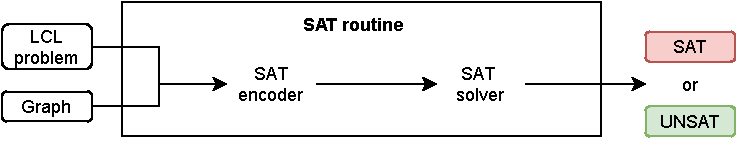
\includegraphics[]{diagrams/implementation_idea_diagram2.pdf}
\caption{The SAT routine. When given a multigraph and an LCL problem, it checks if a valid labeling exists.}
\label{fig:implementation:1}
\end{figure}

We repeat the routine for each multigraph, as shown in the Algorithm~\ref{alg:counterexample_finder}, and terminate early if the result is UNSAT.
This is illustrated in Figure~\ref{fig:implementation:2}.

\begin{figure}[H]
\centering
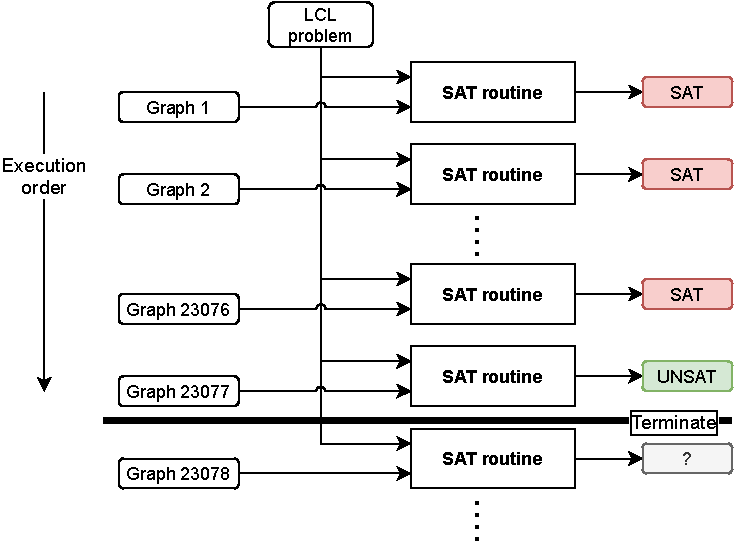
\includegraphics[]{diagrams/implementation_idea_diagram3.pdf}
\caption{An example of an execution of multiple SAT routines. Execution terminates at the 77th multigraph, when first UNSAT is encountered.}
\label{fig:implementation:2}
\end{figure}

Now we discuss how we encode the SAT problem, given that we have an LCL problem $\Pi=(A, P, \Sigma)$ from class $(\Delta, \delta, \lambda)$, and a connected $(\Delta, \delta)$-biregular multigraph $G=(V,E)$, where the parts of vertices are $V_A$ and $V_P$.
Each active node can have possibly any label configuration from $A$ (respectively passive nodes and $P$), and there are always as many ways to label a label configuration as there are permutations of the label configuration.
Let $\operatorname{Perm}(A)$ and $\operatorname{Perm}(P)$ be the sets of all permutations of label configurations in sets $A$ and $P$, respectively.

We define variables $L_{A,u,v,l}$ for each incident edge $(u, v)$ of an active node $u$, for each possible label $l \in \Sigma$.
Similarly, we define variables $L_{P,u,v,l}$ for each incident edge $(u, v)$ of a passive node $u$, for each possible label $l \in \Sigma$.
We also define variables $R_{A, u, p}$ for each permutation of each label configuration in $A$, for each active node $u$.
Similarly, we define variables $R_{P, u, p}$ for each permutation of each label configuration in $P$, for each passive node $u$.
In all of these variables, $A$ and $P$ denote that the node $u$ is from $V_A$ and $V_P$, respectively.

\renewcommand{\labelenumi}{\arabic{enumi}.}
\renewcommand{\labelenumii}{\arabic{enumi}\alph{enumii}.}
We have 3 conditions for our encoding.
Each condition is applied twice, once for active nodes and once for passive nodes.
\begin{enumerate}
\item
  Each node has to agree with their adjacent node on the labels of each edge between them.
  \begin{enumerate}
  \item
    For each $e=(u, v)\in E, u\in V_A$, for each label pair $(l_1, l_2), l_1, l_2 \in \Sigma, l_1 \neq l_2$, we require that at most one of the variables $L_{A,u,v,l_1}, L_{P,v,u,l_2}$ is true, i.e. clause $(\neg L_{A,u,v,l_1} \lor \neg L_{P,v,u,l_2})$.
    \label{enu:sat_conditions:1a}
  \item
    For each $e=(u, v)\in E, u\in V_P$, for each label pair $(l_1, l_2), l_1, l_2 \in \Sigma, l_1 \neq l_2$, we require that at most one of the variables $L_{P,u,v,l_1}, L_{A,v,u,l_2}$ is true, i.e. clause $(\neg L_{P,u,v,l_1} \lor \neg L_{A,v,u,l_2})$
    \label{enu:sat_conditions:1b}
  \end{enumerate}
\item
  Each node can only be applied one permutation of label configurations.
  \begin{enumerate}
  \item
    Let us fix an active node $u \in V_A$.
    For each permutation $p \in \operatorname{Perm}(A)$, we require that only one $R_{A, u, p}$ is true, i.e. clause $(R_{A, u, p_1} \lor R_{A, u, p_2} \lor \dotsm \lor R_{A, u, p_{|\operatorname{Perm}(A)|}})$ for requiring at least one permutation,
    and clauses
    $ (\neg R_{A, u, p_i} \lor \neg R_{A, u, p_j})$ where $i, j \in \{1, ..., |\operatorname{Perm}(A)|\}, i < j$,
    for requiring at most one permutation.
    We repeat this for each active node $u \in V_A$.
    \label{enu:sat_conditions:2a}
  \item
    Let us fix a passive node $u \in V_P$.
    For each permutation $p \in \operatorname{Perm}(P)$, we require that only one $R_{P, u, p}$ is true, i.e. clause $(R_{P, u, p_1} \lor R_{P, u, p_2} \lor \dotsm \lor R_{P, u, p_{|\operatorname{Perm}(P)|}})$ for requiring at least one permutation,
    and clauses
    $ (\neg R_{P, u, p_i} \lor \neg R_{P, u, p_j})$ where $i, j \in \{1, ..., |\operatorname{Perm}(P)|\}, i < j$,
    for requiring at most one permutation.
    We repeat this for each passive node $u \in V_P$.
    \label{enu:sat_conditions:2b}
  \end{enumerate}
\item
  A permutation of label configurations implies that a node labels its incident edges according to the permutation.
  \begin{enumerate}
  \item
    Let us fix an active node $u \in V_A$.
    For each permutation $p \in \operatorname{Perm}(A)$, for each label $l_i \in p, 1 \leq i \leq \Delta$, we require that $R_{A, u, p}$ implies $L_{A,u,v_i,l_i}$, where $v_i$ is the $i$-th adjacent passive node of active node $u$.
    That is, we get a clause $(\neg R_{A, u, p} \lor L_{A,u,v_i,l_i})$.
    We repeat this requirement for each active node $u \in V_A$.
    \label{enu:sat_conditions:3a}
  \item
    Let us fix a passive node $u \in V_P$.
    For each permutation $p \in \operatorname{Perm}(P)$, for each label $l_i \in p, 1 \leq i \leq \delta$, we require that $R_{P, u, p}$ implies $L_{P,u,v_i,l_i}$, where $v_i$ is the $i$-th adjacent active node of passive node $u$.
    That is, we get a clause $(\neg R_{P, u, p} \lor L_{P,u,v_i,l_i})$.
    We repeat this requirement for each passive node $u \in V_P$.
    \label{enu:sat_conditions:3b}
  \end{enumerate}
\end{enumerate}

Based on the above conditions and clauses, we encode the SAT by forming a conjunction of the clauses.
Formatting the problem as DIMACS CNF can be done with a simple mapping from the variables to unique positive integers, or negative integers in case of a negated variable.
It is quite trivial, therefore we do not discuss more about it.
After obtaining the SAT problem in DIMACS CNF, we feed the problem into a SAT solver, as showed in Figure~\ref{fig:implementation:1}.
In our implementation, we use the SAT solver called Kissat~\cite{BiereFazekasFleuryHeisinger-SAT-Competition-2020-solvers, Kissat}, which is the winner in the main track of the SAT Competition 2020~\cite{SatCompetition2020}.


\subsection{Generating LCL Problems} \label{sec:implementation:generating_lcl_problems}

When we generate LCL problems, we generate whole class of LCL problems.
A class of LCL problems is a set of LCL problems where the problems share common attributes.
The attributes are the values of a triple $(\Delta, \delta, \lambda)$, where $\Delta$ and $\delta$ are the sizes of label configurations in $A$ and $P$, respectively, and $\lambda$ is the size of $\Sigma$ i.e. the number of labels.

The set of all possible label configurations is a $k$-combination with repetitions, where $k$ is the size of a label configuration.
Let us call the function of $k$-combination with repetitions as $\operatorname{comb}(k, \Sigma)$.
For example, if $\Delta$ is 2, $\Sigma=\{A, B\}$ and $\lambda$ is 2, then the set of all possible label configurations is
$$ \operatorname{comb}(\Delta, \Sigma) = \{ \{A, A\}, \{A, B\}, \{B, B\} \}. $$

The set of all possible sets of label configurations is a power set of the set of all possible label configurations, excluding an empty set.
Let us call this power set without an empty sets as a function $\operatorname{pow}(d, S)$, where $d$ is the size of a label configuration, and $S$ is the set of all possible label configurations.
For example, the power set of the above example excluding an empty set is
\begin{align*}
  \operatorname{pow}(\Delta, \operatorname{comb}(\Delta, \Sigma)) =  \{&\{\{A, A\}\}, \\
    &\{\{A, B\}\}, \\
    &\{\{B, B\}\}, \\
    &\{\{A, A\}, \{A, B\}\}, \\
    &\{\{A, A\}, \{B, B\}\}, \\
    &\{\{A, B\}, \{B, B\}\}, \\
    &\{\{A, A\}, \{A, B\}, \{B, B\}\} \}.\\
\end{align*}

The set of all LCL problems of class $(\Delta, \delta, \lambda)$ is a Cartesian product
$$ \operatorname{comb}(\Delta, \Sigma) \times \operatorname{comb}(\delta, \Sigma),$$
where $\Sigma$ is any set of labels of length $\lambda$.
In our implementation, we use the upper-case alphabet as $\Sigma$.
The elements are pairs $(A, P)$, where $A$ is the set of all allowed label configurations for active nodes, and $P$ is the set of all allowed label configurations for passive nodes.

Now that we know how to generate a class of LCL problems, we show the number of elements in some chosen classes in Table~\ref{tbl:lcl_problem_classes}.
In the table, we also show the numbers of \emph{purged} and \emph{normalized} problems for each chosen class.
These are the optimizations that reduce the size of problems we have to process through in our implementation, and we discuss them next.

\begin{table}[H]
  \centering
  \begin{tabular}{r|rrr}
    \toprule
    $(\Delta, \delta, \lambda)$ & Problems & Purged problems & Purged and normalized\\
    \midrule
    (1,1,1)& 1 & 1 & 1 \\
    (1,1,2)& 9 & 3 & 2 \\
    (2,1,2)& 21 & 7 & 5 \\
    (2,2,2)& 49 & 27 & 18 \\
    (3,2,2)& 105 & 67 & 38 \\
    (4,2,2)& 217 & 147 & 84 \\
    (4,3,2)& 465 & 379 & 200 \\
    (4,4,2)& 961 & 843 & 446 \\
    (6,6,2)& 16129 & 15627 & 7926 \\
    (2,2,3)& 3969 & 2103 & 419 \\
    (3,2,3)& 64449 & 44343 & 7735 \\
    (3,3,3)& 1046529 & 962871 & 162299 \\
    \vdots & \vdots\\
    \bottomrule
  \end{tabular}
  \caption{%
    The number of LCL problems in different problem classes.
  }
  \label{tbl:lcl_problem_classes}
\end{table}

Purging is an operation, where an LCL problem is cut down from label configurations that are redundant, in a sense that they cannot possibly be in a valid configuration, no matter what.
These redundant label configurations are found by forming a list of labels that appear in both sets $A$ and $P$.
Then we remove each label configuration from both sets, that have some other labels than what was in the list.

For example, if $A=\{\{A, A\}, \{A, B\}, \{B, B\}\}$ and $P=\{\{A, A\}, \{A, C\}, \{C, C\}\}$, then the labels in $A$ are $\{A, B\}$ and labels in P are $\{A, C\}$.
The labels that appear in both $A$ and $P$, i.e.  $\{A, B\} \cup \{A, C\} $ is $\{A\}$.
Thus, we remove all label configurations from both $A$ and $P$ that contain any other label than $A$.
In the end, we get $A=\{\{A, A\}\}$ and $P=\{\{A, A\}\}$.


Normalizing an LCL problem is an operation of renaming the labels with a permutation such that the resulting problem is the minimum of all permutated problems.
Here, we assume that each label in a label configuration is represented in lexicographic order, and each label configuration is also represented in lexicographic order in both sets $A$ and $P$.
We also assume a common set of labels, the upper-case alphabet.
The total order of two LCL problems is the lexicographic order.
That is, the total order of problems $\Pi_1=(A_1, P_1, \Sigma_1), \Pi_2=(A_2, P_2, \Sigma_2)$ from problem class $(\Delta, \delta, \lambda)$ is $\Pi_1 < \Pi_2$ if and only if $A_1 < A_2$ or $(A_1 = A_2 \text{ and } P_1 < P_2)$.
The result of normalization is an LCL problem in its \emph{canonical form}.
After normalizing any two isomorphic LCL problems, their appearance is identical.

For example, the problems $$\Pi_1=(\{\{B, B\}\}, \{\{A, C\}, \{C,C\}\}, \Sigma), \Pi_2=(\{\{D, D\}\}, \{\{A,A\},\{E, A\}\}, \Sigma)$$ after normalization look like $$\Pi_1'=(\{\{A, A\}\}, \{\{B,B\},\{B, C\}\}, \Sigma), \Pi_2'=(\{\{A, A\}\}, \{\{B,B\},\{B, C\}\}, \Sigma)$$ (denoted by a prime).

In our implementation, we first generate all LCL problems.
Then we use the purge operation for each LCL problem, and remove problems that have an empty set of label configurations.
Finally, we normalize each problem, and remove duplicates.
The amount of problems after purging and normalizing can be seen in Table~\ref{tbl:lcl_problem_classes}.



\subsection{Optimizations} \label{sec:implementation:optimizations}
In this section, we will discuss some optimizations used in the implementation that we have not yet mentioned in previous sections.
The optimizations we discuss here briefly, utilizes either parallelization or caching.

When we generate graphs with genbg, we actually do it in parallel using multiple threads.
The tool can be given arguments \codee{r/m} so that it only generates subset \codee{r} from subsets between $0$ and \codee{m}$-1$.
For example, to split it evenly between 4 threads, we give the first thread 0/4, the second thread 1/4, the third thread 2/4, and finally the fourth thread 3/4.
We then pipe the results to multig in each thread in parallel.
This makes the time it takes to generate the graphs roughly $t$-times faster, where $t$ is the number of threads used, assuming that there are $t$ available cores in the system.

When multigraphs are generated, we can optionally save them into a database.
Already generated multigraphs can be fetched from the database when needed, nearly for free in terms of time.
Similarly, LCL problems can also be saved into the database, and automatically fetched from there.

In our implementation, finding counterexamples for multiple LCL problems is done in parallel, utilizing all logical cores of the system.
This can be done quite trivially, as different instances of finding counterexamples do not really depend on each other.
They only depend on the multigraphs to generate SAT problems, which can be accessed safely with read-only access.


\clearpage
%!tex root = ../main.tex

\section{Results} \label{sec:results}
%TODO Show all results that have been found while doing the research, like different problems that have now new lower bounds.

%\begin{figure}[H]
% \centering
% \includegraphics[]{example-image-duck}
% \caption{\todo{Illustration of k-lift using Theorem \ref{lem:lcl_unsolvability:from_klift_to_simple}}}
% \label{fig:duck2}
%\end{figure}

\clearpage
%!tex root = ../main.tex

\section{Conclusion} \label{sec:conclusion}

I present a novel algorithm that can detect if an LCL problem does not have a solution in finite connected $(\Delta, \delta)$-biregular multigraphs.
Then I show that if the problem does not have a solution in the graph family, it is also unsolvable in the PN model.

I also prove that if an LCL problem is not solvable in the PN model, it cannot be solved in constant time in the LOCAL model.
Thus, our algorithm can automatically prove that an LCL problem is not solvable in constant time in the LOCAL model i.e.\ giving it a lower bound of $\Omega(\log^* n)$.

In order to automatically find new lower bounds in practice, I present an implementation of the algorithm.
With the implementation, I find 9 LCL problems with new lower bound and as a consequence, the problem
\begin{align*}
    A&=\text{AAA BBC},\\
    P&=\text{AB AC BB CC},
\end{align*}
is now classified with a tight bound of $\Theta(\log^* n)$.
The implementation uses the state-of-the-art graph generation and SAT solving software, in addition to parallelization, to be able to classify large LCL problem classes.

\subsection{Future Work}

Concerning the performance of the implementation, there is still room for improvements.
The graph generation is a huge bottleneck and generating large number of graphs causes the implementation to terminate.
If this can be solved, the implementation could classify problems using higher degree multigraphs.
The implementation in its current state does not fully support high performance computing.
With a support for high performance computing, we could potentially find even more interesting results than what we have found.
We could also analyze more closely the problems and multigraphs in which the problems are unsolvable.
This could reveal some general patterns or ideas for more classifiers.


\clearpage
\thesisbibliography
\printbibliography

%% In case I need an appendix or two, uncomment the following lines.

%\clearpage
%\thesisappendix
%\section{First example appendix\label{AppendixA}}
%\clearpage
%\section{Second example appendix\label{AppendixB}}


\end{document}
